% This final source is assembled into one standalone TeX file.
\documentclass[11pt,a4paper]{article}
\usepackage[T1]{fontenc}
\usepackage{lmodern,microtype,amsmath,amssymb,amsthm,mathtools}
\usepackage[margin=24mm,headheight=15pt]{geometry}
\usepackage{booktabs,array,xcolor,fancyhdr,titlesec,fancyvrb,tikz}
\usepackage[colorlinks=true,linkcolor=teal!65!black,citecolor=teal!65!black,urlcolor=teal!65!black]{hyperref}
\definecolor{ink}{HTML}{15364A}
\definecolor{accent}{HTML}{007C78}
\titleformat{\section}{\Large\sffamily\bfseries\color{ink}}{\thesection}{.55em}{}
\titleformat{\subsection}{\large\sffamily\bfseries\color{accent}}{\thesubsection}{.55em}{}
\newtheorem{theorem}{Theorem}[section]
\newtheorem{lemma}[theorem]{Lemma}
\newtheorem{proposition}[theorem]{Proposition}
\newtheorem{corollary}[theorem]{Corollary}
\theoremstyle{remark}\newtheorem{remark}[theorem]{Remark}
\DeclareMathOperator{\conv}{conv}
\DeclareMathOperator{\vol}{vol}
\DeclareMathOperator{\Vol}{Vol}
\DeclareMathOperator{\inter}{int}
\DeclareMathOperator{\relint}{relint}
\DeclareMathOperator{\diam}{diam}
\DeclareMathOperator{\Flt}{Flt}
\newcommand{\R}{\mathbb R}\newcommand{\Z}{\mathbb Z}\newcommand{\Q}{\mathbb Q}
\newcommand{\fr}[1]{\left\{#1\right\}}\newcommand{\one}{\mathbf1}
\newcommand{\Bopt}{B_*}
\pagestyle{fancy}\fancyhf{}
\fancyhead[L]{\small\sffamily Lattice covering flows: further transfers}
\fancyhead[R]{\small\sffamily Complete proof manuscript}
\fancyfoot[L]{\footnotesize\sffamily Prepared for Keio | 20 November 2026}
\fancyfoot[R]{\small\thepage}
\setlength{\parindent}{1.1em}\setlength{\parskip}{3pt}
\setlength{\emergencystretch}{2em}\raggedbottom
\hypersetup{pdftitle={Lattice Covering Flows: Collinear Interior Points, Higher Minima, and Flatness Obstructions},pdfauthor={Research manuscript prepared for Keio}}

\begin{document}
\noindent{\sffamily\small\bfseries\color{accent} GEOMETRY OF NUMBERS | FURTHER TRANSFERS FROM VMRC [200]}\par\medskip
\noindent{\sffamily\bfseries\fontsize{23}{27}\selectfont\color{ink}\raggedright
Lattice Covering Flows:\\
Collinear Interior Points,\\
Higher Minima, and\\
Flatness Obstructions\par}
\medskip
\noindent{\large\sffamily An all-dimensional partial resolution of Conjecture D,\par
counterexamples at every intermediate index,\par
and sharp free-sum covering products}\par
\medskip
\noindent Research manuscript prepared for Keio\hfill 20 November 2026

\begin{abstract}
We transfer the weighted fractional-part method of VMRC [200] to three
further questions in lattice covering. First, a chord containing $m$
interior lattice points gives an explicit upper bound involving its two
endpoint gaps. It proves the numerical Codenotti--Santos--Schymura
interior-point conjecture in every dimension whenever all $h\ge3$
interior lattice points are collinear. The endpoints need not be lattice
points, and the constant is sharp. Second, we give weighted-simplex
counterexamples to the original covering-minima conjecture at every
intermediate index $i\ge3$, supplementing the previously settled
$i=2$ case. An exact quotient formula and a nonempty interval of real
counterexample parameters are provided. Third, an elementary
max-convolution product inequality, combined with Krivoku\'ca's
direct-sum theorem, proves supermultiplicativity of the covering product
and a sharp bound for arbitrary free sums of weighted terminal
simplices. We also determine every covering minimum of free sums of
paired-weight tetrahedra. Finally, rational shear triangles show that
even optimizing the interior origin cannot compare the discrete surface
bound with lattice width by a dimension-only factor. This obstruction
persists for non-hollow lattice triangles and maximal lattice-free
triangles. The general numerical interior-point conjecture, the
universal covering-product conjecture, and a linear flatness bound
remain unresolved here. Full proofs of the transfer tools and the
previous paired-tetrahedron input are included.
\end{abstract}

\section{Questions, conventions, and exact scope}
\label{r3:intro}

For a full-dimensional compact convex body $K\subset\R^d$ and a
full-rank lattice $\Lambda$, set
\[
 \mu(K,\Lambda)=\inf\{\rho\ge0:\rho K+\Lambda=\R^d\}.
\]
Thus the covering problem concerns all points of space under lattice
translates of a dilated body. A lattice polytope is \emph{non-hollow}
if its interior contains a lattice point. Covering radius is unchanged
by translating the body, is inversely homogeneous under positive
dilation, and is invariant under simultaneous invertible linear changes
of body and lattice. Every section or quotient below uses its actual
induced lattice, including when selected vertices generate a proper
sublattice.

The $i$th covering minimum is the least dilation whose lattice
arrangement meets every affine subspace of codimension $i$. We use
the standard quotient characterization \cite[Section 1]{CSS}:
\begin{equation}\label{intro:quotient}
 \mu_i(K,\Lambda)=\max_A\mu(AK,A\Lambda),
\end{equation}
where $A$ ranges over rank-$i$ quotients with lattice-rational kernel.
We put $\mu_0=0$. With $\Lambda^*$ the dual lattice, the lattice width is
\[
 w(K,\Lambda)=\min_{0\ne z\in\Lambda^*}
  \left(\max_{x\in K}\langle z,x\rangle-
        \min_{x\in K}\langle z,x\rangle\right)=\mu_1(K,\Lambda)^{-1}.
\]
The flatness constant can be written
$\Flt(d)=\sup_{K,\Lambda}\mu(K,\Lambda)w(K,\Lambda)$.
Our final obstruction concerns one proposed upper estimate for this
product, not a counterexample to flatness itself.

For positive weights define the weighted terminal simplex
\begin{equation}\label{r3:weighted-simplex}
 S_n(\omega)=\conv\{-\omega_0\one_n,
                       \omega_1e_1,\ldots,\omega_ne_n\},
 \qquad T_n=S_n(1,\ldots,1).
\end{equation}
For bodies in complementary subspaces, their free direct sum is
$K\oplus L=\conv((K,0)\cup(0,L))$. We always assume the origin is
interior to each summand when using free-sum gauges and volume formulas.

\subsection{The existing conjectures being tested}

The numerical part of CSS Conjecture D \cite{CSS} is
\begin{equation}\label{r3:conjectureD}
 \mu(P,\Lambda)\le\frac{d-1}{2}+\frac1{h+1},
 \qquad h=|\inter P\cap\Lambda|\ge1.
\end{equation}
The original conjecture additionally proposed equality classifications.
Only its numerical inequality is at issue in our positive collinear
result; no full equality classification is asserted. CSS proved the
numerical inequality for all lattice polygons. Our proof extends a
specified class to all dimensions.

For $\omega_0\le\cdots\le\omega_n$, the original weighted
covering-minima conjecture \cite[Conjecture 5.3]{CSS}, repeated in
\cite[Conjecture 5.3]{Krivokuca}, predicts
\begin{equation}\label{r3:weighted-conjecture}
 \mu_i(S_n(\omega))=
 \frac{\sum_{0\le j<k\le i}(\omega_j\omega_k)^{-1}}
      {\sum_{j=0}^i\omega_j^{-1}}.
\end{equation}
Its endpoint cases $i=1,n$ are established results. The intermediate
claims are refuted here by explicit quotients, supplementing our
earlier exact $i=2$ family.

The universal covering-product conjecture, called Conjecture F in
\cite{CSS}, asks for
\begin{equation}\label{r3:product-conjecture}
 \mathcal F_d(K,\Lambda):=
 \frac{\vol_d(K)}{\det\Lambda}\prod_{i=1}^d\mu_i(K,\Lambda)
 \ge\frac{d+1}{2^d}.
\end{equation}
Here $\vol_d$ is ordinary Euclidean volume, so no factorial is hidden
in this definition. Our theorem gives a closure principle for arbitrary
free sums and proves a stronger sharp constant on a specified family;
it does not resolve \eqref{r3:product-conjecture} for arbitrary bodies.

\subsection{Relation to the previous 23-page manuscript}

This is a separate follow-up to \cite{TransferTwo}. The positive
all-dimensional collinear theorem, the $i\ge3$ counterexample intervals,
the free-sum product principle, and the optimized-origin obstruction
are the developments of this investigation. The exact two-part flow
formula and the paired-tetrahedron profile were established in that
earlier manuscript. Their proofs are reproduced here so that the new
consequences do not require an unavailable auxiliary calculation.
The remaining results of the earlier manuscript are not all reprinted.

The core flow estimate and the non-hollow bound are from VMRC [200]
\cite{VMRC200}; their proofs are reproduced in Section~\ref{sec:tools}.
The direct-sum convolution theorem and the single weighted-simplex
covering-product bound are explicitly credited to prior literature.
Mathematical proofs below stand independently of the finite searches.
No assertion of historical priority or completed external peer review
is made.


\section{Exact transfer tools from fractional-part flows}
\label{sec:tools}
For $0\in\inter P$, write
$g_P(x)=\inf\{\rho\ge0:x\in\rho P\}$ for its gauge.
The following lemmas reproduce the needed machinery of VMRC [200]
\cite{VMRC200}, so the applications can be checked within this text.

\begin{lemma}[Exact weighted gauge]\label{tool:gauge}
Let $u_0,\ldots,u_d$ generate the lattice $\Lambda$, and let their
column matrix $U$ have rank $d$ and kernel $\R q$, where
$q\in\Z_{>0}^{d+1}$. For positive $c_j$ set
$P=\conv(u_0/c_0,\ldots,u_d/c_d)$. Then, for every $x=Ut$,
\begin{equation}\label{tool:gaugeeq}
 \min_{z\in\Lambda}g_P(x-z)
 =\min_{s\in[0,1)}\sum_{j=0}^dc_j\fr{t_j+q_js}.
\end{equation}
Consequently the covering radius is the maximum of the right side
over all phases $t$.
\end{lemma}
\begin{proof}
The positive relation puts zero in the interior of $P$.
Every lattice vector is $Un$ for $n\in\Z^{d+1}$, and every
coefficient representation of $x-Un$ is $t-n+sq$.
Its gauge is the infimum of $\sum_jc_j(t_j-n_j+sq_j)$ over these
representations with nonnegative coefficients. For fixed $s$,
the largest allowed $n_j$ is $\lfloor t_j+sq_j\rfloor$, which
minimizes the positive cost. Interchanging the infima over $s,n$
therefore gives the stated fractional parts. The result is
one-periodic and has positive slope between finitely many downward
jumps, so the minimum is attained. The lattice gauge distance is
continuous on the compact quotient torus; its maximum is the
covering radius and is attained as well.
\end{proof}

\begin{lemma}[Jump-square bound and equality]\label{tool:jump}
For positive integers $q_j$, positive real $c_j$, and arbitrary
phases $t_j$, put
\[
 F(s)=\sum_jc_j\fr{t_j+q_js},\qquad C=\sum_jq_jc_j.
\]
Then
\begin{equation}\label{tool:bound}
 \min_sF(s)\le B(q,c):=
 \frac12\sum_jc_j-\frac{\sum_jq_jc_j^2}{2C}.
\end{equation}
Equality holds exactly when all coordinate crossings are distinct
and all post-jump values equal $B(q,c)$.
\end{lemma}
\begin{proof}
Group simultaneous crossings into events $e$ with total jump $J_e$.
Between events $F'=C$, while
$\int_0^1F=\tfrac12\sum_jc_j$ and $\sum_eJ_e=C$.
The change of $F^2$ at $e$ is $-2J_eF(e)-J_e^2$, using its
right-continuous value. Periodicity thus gives
\[
 \frac1C\sum_eJ_eF(e)
 =\frac12\sum_jc_j-\frac1{2C}\sum_eJ_e^2
 \le B(q,c).
\]
The first side is a convex combination of post-jump values.
The inequality follows from positivity, because grouped squared
jumps are at least the sum of the individual squares.
Equality requires all values in the convex combination to be the
minimum and every group to have one crossing; these conditions
also suffice.
\end{proof}

\begin{remark}[Individual jumps at coincident times]\label{tool:individual}
For exact deficit calculations, simultaneous crossings may instead
be recorded in any specified sequential order, with zero time
between them. Let $w_e$ be the individual jump size and let $H_e$
be its formal intermediate post-jump value. These values are all
at least the actual final post-jump value. Telescoping the individual
changes of $F^2$ remains exact, and for $M=\min F$ it yields
\begin{equation}\label{tool:deficit}
 M=B(q,c)-\frac1C\sum_e w_e(H_e-M),\qquad H_e-M\ge0.
\end{equation}
This convention accounts for cross terms of coincident jumps; it
does not identify intermediate values with the right-continuous
value of $F$ at that time.
\end{remark}

\begin{corollary}[Upper bound without a lattice-generation assumption]
\label{tool:upper}
If integer columns $u_0,\ldots,u_d$ span $\R^d$ and have a positive
integer relation $q$, then for $P=\conv(u_j/c_j)$,
\[
 \mu(P,\Lambda)\le B(q,c),
\]
even when the columns are nonprimitive or generate a proper
sublattice of $\Lambda$.
\end{corollary}
\begin{proof}
For $x=\sum_jt_ju_j$, the vector
$z(s)=\sum_j\lfloor t_j+sq_j\rfloor u_j$ lies in $\Lambda$ and
\[
 x-z(s)=\sum_jc_j\fr{t_j+sq_j}(u_j/c_j).
\]
The coefficients are nonnegative. At a minimizing event their
sum is at most $B(q,c)$, so the residual lies in $B(q,c)P$.
This works for every real $x$. Only the exact reverse direction
in Lemma~\ref{tool:gauge} needs lattice generation.
\end{proof}

\begin{lemma}[Section and quotient]\label{tool:section}
Let $0\in\inter K$ and let $L$ be a rational linear subspace.
For the quotient map $\pi$,
\[
 \mu(K,\Lambda)\le
 \mu(K\cap L,\Lambda\cap L)+\mu(\pi K,\pi\Lambda).
\]
\end{lemma}
\begin{proof}
Take numbers $a,b$ strictly larger than the section and quotient
radii. For any $x$, quotient covering supplies $y\in bK$ and
$z\in\Lambda$ with $x-y-z\in L$. Section covering writes this
residual as $w+v$, where $w\in\Lambda\cap L$ and $v\in a(K\cap L)$.
Thus $x\in z+w+(a+b)K$ by convexity. Let $a,b$ decrease to their
radii. This is the standard inequality \cite[Lemma 2.1]{CSS}.
\end{proof}

\begin{proposition}[The non-hollow bound from the transfer]
\label{tool:nonhollow}
Every lattice $d$-polytope with an interior lattice point has
covering radius at most $d/2$.
\end{proposition}
\begin{proof}
For a lattice simplex with zero in its interior, apply
Corollary~\ref{tool:upper} to its actual vertices and all $c_j=1$.
The positive integer relation exists because the vertex matrix is
integral and has a positive one-dimensional kernel. The resulting
bound is $(d+1)/2-1/2=d/2$.

For a polytope, translate an interior lattice point to zero and
choose an inclusion-minimal set of vertices whose convex hull
contains zero. It is a simplex $S$ with zero in its relative
interior. Let $r=\dim S$ and $L=\operatorname{span}S$. If $r=d$,
monotonicity gives the simplex bound. Otherwise $\pi P$ is a
non-hollow lattice $(d-r)$-polytope, and induction together with
Lemma~\ref{tool:section} gives
\[
 \mu(P)\le\mu(P\cap L)+\mu(\pi P)
 \le\mu(S)+(d-r)/2\le d/2.
\]
The one-dimensional base case is the interval statement. This
reproduces the required consequence of [200] with the actual
ambient lattice throughout.
\end{proof}



\begin{proposition}[The all-one relation and terminal covering minima]
\label{tool:terminal}
For arbitrary positive weights,
\begin{equation}\label{tool:weighted-radius}
 \mu(S_d(\omega),\Z^d)=
 \frac{\sum_{0\le j<k\le d}(\omega_j\omega_k)^{-1}}
      {\sum_{j=0}^d\omega_j^{-1}}.
\end{equation}
Moreover, $\mu_i(T_n,\Z^n)=i/2$ for all $1\le i\le n$.
\end{proposition}
\begin{proof}
For the first assertion use columns $-\one_d,e_1,\ldots,e_d$,
relation $q=(1,\ldots,1)$, and $c_j=1/\omega_j$ in
Lemma~\ref{tool:gauge}. These columns generate $\Z^d$.
The jump bound is
$B=(\sum c_j)/2-(\sum c_j^2)/(2\sum c_j)
=\sum_{j<k}c_jc_k/\sum c_j$.
To attain it, arrange the $d+1$ distinct jumps in any cyclic order
and put a time gap $c_j/C$ immediately before the jump of size $c_j$,
where $C=\sum c_j$. The gaps are positive and sum to one.
Choose the corresponding phases. Every rise is exactly cancelled
by the next jump, so all post-jump values are equal. The jump-square
identity forces their common value to be $B$. The exact gauge
formula proves \eqref{tool:weighted-radius}, which is the established
formula of \cite[Theorem 1.4]{CSS}, here recovered from the flow.

Every rational rank-$i$ quotient of $T_n$ is a non-hollow lattice
$i$-polytope in the projected lattice, so
Proposition~\ref{tool:nonhollow} gives $\mu_i(T_n)\le i/2$.
Projection onto the first $i$ coordinates gives $T_i$, with any
remaining vertices projecting to zero. The formula just proved
gives $\mu(T_i)=i/2$, proving the opposite inequality.
\end{proof}

\begin{lemma}[Free-sum gauges, radii, and volume]
\label{tool:freesum}
Let $K\subset\R^p$ and $L\subset\R^q$ contain zero in their
interiors, with lattices $\Lambda$ and $\Gamma$. Then
\begin{align*}
 g_{K\oplus L}(x,y)&=g_K(x)+g_L(y),\\
 \mu(K\oplus L,\Lambda\oplus\Gamma)
 &=\mu(K,\Lambda)+\mu(L,\Gamma),\\
 \frac{\vol_{p+q}(K\oplus L)}{\det(\Lambda\oplus\Gamma)}
 &=\frac{p!q!}{(p+q)!}
   \frac{\vol_p(K)}{\det\Lambda}
   \frac{\vol_q(L)}{\det\Gamma}.
\end{align*}
\end{lemma}
\begin{proof}
Membership in the free sum is equivalent to
$g_K(x)+g_L(y)\le1$, giving the first identity.
The two lattice minimizations separate, as do their maxima on the
product torus, proving the second. For the last identity, apply a
linear change putting the lattice product into standard coordinates;
both sides have the same determinant covariance. In these coordinates
the section at $x\in K$ is $(1-g_K(x))L$, so its volume is
$(1-g_K(x))^q\vol_q(L)$. Since
$\vol_p\{x:g_K(x)\le t\}=t^p\vol_p(K)$, integration gives
\[
 \vol_{p+q}(K\oplus L)
 =\vol_p(K)\vol_q(L)\,p\int_0^1t^{p-1}(1-t)^q\,dt
 =\frac{p!q!}{(p+q)!}\vol_p(K)\vol_q(L).
\]
\end{proof}


\section{A quantitative bound from a line of interior lattice points}
\label{r3d:section}

The weighted form of the transfer is useful even when one vertex of an
auxiliary simplex is not a lattice point.  This observation removes the
lattice-endpoint restriction from a substantially larger class of the
numerical interior-point conjecture.  All covering radii below are taken
in the actual ambient lattice; no generation hypothesis on the chosen
directions is imposed.  The numerical conjecture for lattice polygons,
including their collinear-interior-point case, was already proved in
\cite[Theorem 6.3]{CSS}; the argument below applies in every dimension.

\begin{lemma}[Primitive-direction form of the upper bound]
\label{r3d:primitive}
Let $S=\conv(v_0,\ldots,v_r)$ be an $r$-simplex with $0\in\inter S$,
and write $v_i=\lambda_i u_i$, where $\lambda_i>0$ and the $u_i$ are
primitive vectors of a full-rank lattice $\Gamma$.  If
$\alpha_0,\ldots,\alpha_r$ are the barycentric coordinates of zero,
then
\begin{equation}\label{r3d:primitiveeq}
 \mu(S,\Gamma)\le
 \frac12\sum_{i=0}^{r}\frac{1-\alpha_i}{\lambda_i}.
\end{equation}
The lengths $\lambda_i$ may be nonintegral.
\end{lemma}
\begin{proof}
The integer matrix with columns $u_i$ has a one-dimensional positive
kernel, so choose a positive integer kernel vector $q$.  Put
$c_i=1/\lambda_i$ and $C=\sum_iq_ic_i$.  The barycentric relation gives
$\alpha_i=q_ic_i/C$.  Consequently Corollary~\ref{tool:upper} gives
\[
 \mu(S,\Gamma)
 \le\frac12\sum_i c_i-\frac{1}{2C}\sum_iq_ic_i^2
 =\frac12\sum_i\frac{1-\alpha_i}{\lambda_i}.
\]
This is the primitive-direction form of the discrete surface-area
bound from \cite{VMRC200}.  The proof uses only that the $u_i$ lie in
$\Gamma$, not that they generate it.
\end{proof}

\begin{lemma}[One rational endpoint as an auxiliary vertex]
\label{r3d:ray}
Let $P$ be a lattice $d$-polytope in a full-rank lattice $\Lambda$,
with $0\in\inter P$.  Let $u\in\Lambda$ be primitive and suppose
\[
 P\cap\R u=[-\beta u,\gamma u],\qquad \beta,\gamma>0.
\]
Then
\begin{equation}\label{r3d:rayeq}
 \mu(P,\Lambda)\le
 \frac{d-1}{2}+\frac{1+\beta}{2(\beta+\gamma)}.
\end{equation}
Neither endpoint is required to be a lattice point.
\end{lemma}
\begin{proof}
Set $w=-\beta u$ and $v=\gamma u$.  Choose a facet $F$ of $P$
containing $w$, and choose an inclusion-minimal set of vertices
$w_1,\ldots,w_r$ of $F$ whose convex hull contains $w$.  These vertices
are affinely independent and $w$ belongs to the relative interior of
their convex hull.  A supporting hyperplane of $F$ cannot contain
$v$: otherwise it would contain the open segment from $w$ to $v$,
including the interior point zero.  Thus
\[
 S=\conv(v,w_1,\ldots,w_r)
\]
is an $r$-simplex, $S\subseteq P$, and $0\in\operatorname{relint}S$.
Its linear span $L$ is rational, since it is spanned by $u$ and the
lattice vectors $w_i$.  The vector $u$ remains primitive in
$\Lambda\cap L$.

The barycentric coefficient of $v$ at zero is
\[
 \alpha_v=\frac{\beta}{\beta+\gamma},
\]
because zero divides the segment from $w$ to $v$ in that ratio.
The primitive length of $v$ is $\gamma$, while every $w_i$ has an
integer primitive length at least one.  Lemma~\ref{r3d:primitive}
therefore implies
\begin{align*}
 \mu(S,\Lambda\cap L)
 &\le \frac12\left(r-1+\alpha_v+
                  \frac{1-\alpha_v}{\gamma}\right)\\
 &=\frac{r-1}{2}+\frac{1+\beta}{2(\beta+\gamma)}.
\end{align*}
If $r=d$, monotonicity gives the assertion.  If $r<d$, the quotient
$\pi P$ is a non-hollow lattice $(d-r)$-polytope in $\pi\Lambda$.
The section-and-quotient inequality and the non-hollow bound give
\[
 \mu(P,\Lambda)
 \le \mu(P\cap L,\Lambda\cap L)+\mu(\pi P,\pi\Lambda)
 \le \mu(S,\Lambda\cap L)+\frac{d-r}{2}.
\]
This proves \eqref{r3d:rayeq}.  The use of a nonlattice auxiliary vertex
is legitimate because Lemma~\ref{r3d:primitive} permits real lengths
along primitive lattice directions.
\end{proof}


\begin{figure}[htbp]
\centering
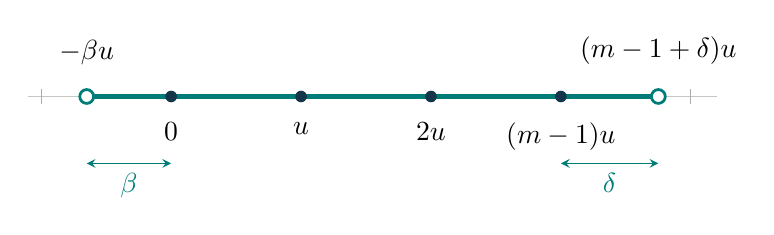
\begin{tikzpicture}[x=1.65cm,y=1cm,>=stealth]
 \draw[gray!45,thin] (-1.1,0)--(4.2,0);
 \draw[accent,line width=1.8pt] (-.65,0)--(3.75,0);
 \foreach \x in {-1,4} {
   \draw[gray!65] (\x,-.09)--(\x,.09);
 }
 \foreach \x in {0,1,2,3} {
   \fill[ink] (\x,0) circle (2.1pt);
 }
 \draw[accent,fill=white,line width=1pt] (-.65,0) circle (2.5pt);
 \draw[accent,fill=white,line width=1pt] (3.75,0) circle (2.5pt);
 \node[below=6pt] at (0,0) {$0$};
 \node[below=6pt] at (1,0) {$u$};
 \node[below=6pt] at (2,0) {$2u$};
 \node[below=6pt] at (3,0) {$(m-1)u$};
 \node[above=8pt] at (-.65,0) {$-\beta u$};
 \node[above=8pt] at (3.75,0) {$(m-1+\delta)u$};
 \draw[<->,accent] (-.65,-.85)--(0,-.85)
       node[midway,below] {$\beta$};
 \draw[<->,accent] (3,-.85)--(3.75,-.85)
       node[midway,below] {$\delta$};
\end{tikzpicture}
\caption{A line section with $m=4$ interior lattice points shown
schematically. The endpoint gaps lie in $(0,1]$. Both ends may be
nonlattice points; the proof uses each end in turn as an auxiliary
simplex vertex.}
\label{fig:line}
\end{figure}

\begin{theorem}[A line of interior lattice points]
\label{r3d:line}
Let $P$ be a lattice $d$-polytope and let an affine lattice line
$\ell$ contain exactly $m\ge2$ points of $\inter P\cap\Lambda$.
Translate and orient the line so that those points are
$0,u,\ldots,(m-1)u$, with $u$ primitive, and write
\[
 P\cap\ell=[-\beta u,(m-1+\delta)u],
 \qquad 0<\beta,\delta\le1.
\]
Then
\begin{equation}\label{r3d:lineeq}
 \boxed{\displaystyle
 \mu(P,\Lambda)\le\frac{d-1}{2}
       +\frac{1+\min\{\beta,\delta\}}
                    {2(m-1+\beta+\delta)}.}
\end{equation}
In particular, if $m\ge3$, then
\begin{equation}\label{r3d:mbound}
 \mu(P,\Lambda)\le\frac{d-1}{2}+\frac{1}{m+1}.
\end{equation}
For $m=2$, the same bound holds whenever
\begin{equation}\label{r3d:twocond}
 2\max\{\beta,\delta\}\ge1+\min\{\beta,\delta\}.
\end{equation}
In particular, it holds for $m=2$ if at least one endpoint of
$P\cap\ell$ is a lattice point.
\end{theorem}
\begin{proof}
The points of the lattice on the line form an arithmetic progression.
Convexity and openness of $\inter P$ show that the interior lattice
points on the line are consecutive.  The absence of one more such
point on either end is exactly $0<\beta,\delta\le1$.

Apply Lemma~\ref{r3d:ray} with $\gamma=m-1+\delta$.  Reversing the
orientation and translating $(m-1)u$ to zero interchanges $\beta$ and
$\delta$.  The smaller of the two bounds is \eqref{r3d:lineeq}.

Put $b=\min\{\beta,\delta\}$ and $c=\max\{\beta,\delta\}$.  The
comparison with the desired interior-point expression is the exact
identity
\begin{equation}\label{r3d:comparison}
 \frac{1}{m+1}-\frac{1+b}{2(m-1+b+c)}
 =\frac{(m-3)(1-b)+2(c-b)}
        {2(m+1)(m-1+b+c)}.
\end{equation}
It is nonnegative for $m\ge3$, since $0<b\le c\le1$.  For $m=2$,
its numerator is $2c-1-b$, giving \eqref{r3d:twocond}.  If one endpoint
is a lattice point, then $c=1$, which satisfies that condition.
\end{proof}

\begin{corollary}[The numerical conjecture for collinear interior points]
\label{r3d:collinear}
Let $P$ be a lattice $d$-polytope whose $h$ interior lattice points
are collinear.  If $h\ge3$, then
\[
 \mu(P,\Lambda)\le\frac{d-1}{2}+\frac{1}{h+1}.
\]
The same conclusion holds for $h=2$ under
\eqref{r3d:twocond}, in particular if the line through the two points
has a lattice endpoint in its intersection with $P$.
\end{corollary}
\begin{proof}
Take $m=h$ in Theorem~\ref{r3d:line}.
\end{proof}

\begin{corollary}[A quantitative strict deficit with two interior points]
\label{r3d:strict}
If a lattice $d$-polytope has at least two interior lattice points,
then $\mu(P,\Lambda)<d/2$. More precisely, for any line in
Theorem~\ref{r3d:line}, with $b=\min\{\beta,\delta\}$ and
$c=\max\{\beta,\delta\}$,
\[
 \frac d2-\mu(P,\Lambda)
 \ge\frac{m-2+c}{2(m-1+b+c)}>0.
\]
\end{corollary}
\begin{proof}
Choose the line through two distinct interior lattice points and
apply \eqref{r3d:lineeq}. Subtract its right side from $d/2$.
The numerator is positive because $m\ge2$ and $c>0$.
\end{proof}

This recovers, with a shorter proof and an explicit geometric deficit,
the strict inequality established in \cite{TransferTwo}. The deficit
here need not equal the conjectured $1/6$ when there are two points;
condition \eqref{r3d:twocond} is still needed for that comparison.

\begin{remark}[Sharpness and what remains outside this result]
\label{r3d:scope}
The uniform constant $1/(m+1)$ is sharp in every dimension: for $d\ge2$,
the direct sum of a standard terminal $(d-1)$-simplex and the lattice interval
$[-1,m]$ has exactly $m$ interior lattice points and covering radius
$(d-1)/2+1/(m+1)$.  In dimension one the interval alone suffices.
These sharp examples are part of the original
conjectured family in \cite{CSS}, not new examples.

For completeness, their interior-point count follows directly from
the free-sum gauge. If $r=d-1\ge1$, the facet description of $T_r$ is
\[
 g_{T_r}(x)=\max\left\{\sum_{j=1}^r x_j,
       \sum_{j=1}^r x_j-(r+1)x_i:1\le i\le r\right\}.
\]
It is integer-valued and at least one on every nonzero lattice
vector. Thus an interior lattice point of $T_r\oplus[-1,m]$ must
have its $T_r$-coordinate zero. Its last coordinate is exactly one
of $0,\ldots,m-1$. There are $m$ such points. The covering-radius
formula follows from Lemma~\ref{tool:freesum} and
Proposition~\ref{tool:terminal}.

The comparison \eqref{r3d:comparison} also gives geometric necessary
conditions for equality in the collinear case.  For $m\ge4$, equality
in \eqref{r3d:mbound} requires $\beta=\delta=1$.  For $m=3$, it
requires $\beta=\delta$.  These are necessary conditions only, not a
classification of the polytopes.

For a polytope with additional interior lattice points off $\ell$,
the theorem gives the bound using the number $m$ on that line;
one cannot replace $m$ by the total number $h$ without another
argument.  The numerical conjecture is therefore not resolved here
for arbitrary noncollinear interior point sets, or for all
two-interior-point polytopes.  The remaining two-point geometry in
this argument is precisely $2c<1+b$.
\end{remark}


\section{The exact two-part discrepancy transfer}
\label{r3:two-part-section}

We reproduce the two-part specialization from \cite{TransferTwo}
with its proof, since it computes the new quotients exactly.
For positive weights $a_1,\ldots,a_d,b$ put
\[
 A=\sum_{j=1}^da_j,\qquad C=2b+A,\qquad
 B=\frac{b+A}{2}-\frac{2b^2+\sum_ja_j^2}{2C},
 \qquad
 \Delta=\min_{I\subseteq\{1,\ldots,d\}}
          \left|A-2\sum_{j\in I}a_j\right|.
\]
The distinguished coordinate has frequency two and weight $b$;
all other coordinates have frequency one.

\begin{theorem}[Exact loss equals weighted partition discrepancy]
\label{tool:two-part}
For this frequency pattern,
\begin{equation}\label{r3:two-part-formula}
 \max_{t}\min_{s\in\R}
 \left(b\fr{t_0+2s}+\sum_{j=1}^da_j\fr{t_j+s}\right)
 =B-\frac{b\Delta}{2C}.
\end{equation}
Whenever the integer columns in Lemma~\ref{tool:gauge} generate the
ambient lattice and have this positive relation, the right side is
their weighted simplex's exact covering radius.
\end{theorem}
\begin{proof}
Shift time so the distinguished jumps occur at $0$ and $1/2$.
At a simultaneous event, record the distinguished jump first and
any singleton jumps immediately afterward. Assign singleton events
at a distinguished time to the following half-period. Let $A_0,A_1$
be the total singleton weights in the two half-periods, and let
$H_0,H_1$ be the formal post-jump heights of the two distinguished
jumps. Since $C/2=b+A/2$,
\[
 H_1-H_0=C/2-A_0-b=(A_1-A_0)/2.
\]
For the actual global minimum $M$, all formal post-jump heights
are at least $M$. Hence
$(H_0-M)+(H_1-M)\ge|A_0-A_1|/2\ge\Delta/2$.
The individual-jump identity \eqref{tool:deficit}, with all remaining
excesses nonnegative, gives $M\le B-b\Delta/(2C)$.

For attainment, choose a minimum-discrepancy partition and name its
heavier part $I_0$. Set $\eta=\Delta/2$, so
$A_0=A/2+\eta$ and $A_1=A/2-\eta$. If $\eta>0$, no item in the
heavier part can have weight strictly between zero and $\eta$:
moving such an item of weight $a$ to the other part would reduce
the discrepancy from $2\eta$ to $2\eta-2a$. In particular there is
an item $a\ge\eta$. If $\eta=0$, both parts are nonempty since
$A>0$, and any item can be used.

Prescribe distinguished post-jump excesses $\eta$ and zero at
times $0$ and $1/2$. In the heavier half-period place the selected
singleton after a gap $(a-\eta)/C$; its jump brings the excess to
zero. Place each remaining singleton after a gap equal to its
weight divided by $C$, and finish with a gap $b/C$ before the
distinguished jump at $1/2$. This half-period has duration
$(A_0-\eta+b)/C=1/2$.

In the lighter half-period start at zero, use gaps $a_j/C$ before
each singleton jump, and finish with a gap $(b+\eta)/C$. Its total
duration is $(A_1+b+\eta)/C=1/2$, and the final distinguished jump
returns to excess $\eta$. An empty lighter part is allowed. A zero
first gap is a simultaneous event with the specified formal order;
its final right-continuous height is zero. Thus the constructed
nonnegative profile attains its minimum excess zero.

Each singleton crosses once and the distinguished coordinate crosses
twice at distance $1/2$, so phases realize precisely these event
times and jumps. Between events the slope is $C$. The resulting
fractional-part flow differs from the prescribed profile by a constant.
The weighted sum of formal post-jump excesses is exactly $b\eta$.
Applying \eqref{tool:deficit} to the realized flow fixes its baseline
at $B-b\eta/C$. This attains the asserted upper bound for all real
phases, without any integrality assumption on the weights.
\end{proof}


% Manuscript fragment; no preamble or bibliography.
% Required bibliography keys: CSS, Krivokuca, TransferTwo, VMRC200.
% Required earlier labels: tool:two-part, tool:terminal.
% Required appendix labels: rr:thm:alln, rr:cor:vector.
% TransferTwo is the preceding 23-page transfer manuscript, in particular
% its Theorem 4.2 and Corollary 4.4 on paired weighted terminal simplices.
% All labels introduced in this fragment have prefix r3m:.

\section{Counterexamples at every intermediate covering index}
\label{r3m:sec-counterexamples}

For $0<\omega_0\le\cdots\le\omega_n$, Codenotti, Santos and Schymura
conjectured that
\begin{equation}
\label{r3m:eq-css-prediction}
 \mu_i(S_n(\omega))
 =
 \frac{\displaystyle\sum_{0\le j<k\le i}
               (\omega_j\omega_k)^{-1}}
      {\displaystyle\sum_{j=0}^{i}\omega_j^{-1}}.
\end{equation}
This is \cite[Conjecture~5.3]{CSS}, repeated as
\cite[Conjecture~5.3]{Krivokuca}.  The endpoint cases $i=1$ and $i=n$
are established in \cite{CSS}.  The preceding transfer manuscript
disproved the branch $i=2$ \cite{TransferTwo}.  We now exhibit
counterexamples for every $i\ge3$, in every ambient dimension $n\ge i+1$.

\begin{theorem}[Exact radius of an explicit quotient simplex]
\label{r3m:thm-quotient-radius}
Let $i\ge2$ be an integer and let $r\ge1$ be real.  Define
\[
 P_i(r)=\operatorname{conv}
  \{-(2,1,\ldots,1),re_1,\ldots,re_i\}\subset\mathbb R^i,
 \qquad
 \delta_i(r)=\min_{0\le m\le i-1}|r+i-1-2m|.
\]
Then
\begin{equation}
\label{r3m:eq-exact-quotient}
 \mu(P_i(r),\mathbb Z^i)=R_i(r)
 :=
 \frac{(2i+1)r+i^2-1-\delta_i(r)}
      {2r(r+i+1)}.
\end{equation}
\end{theorem}

\begin{proof}
Take the primitive integral directions
\[
 u_0=-(2,1,\ldots,1),\qquad u_j=e_j\quad(1\le j\le i).
\]
They generate the full lattice $\mathbb Z^i$, and their primitive
positive relation is
\[
 u_0+2u_1+u_2+\cdots+u_i=0.
\]
The reciprocal vertex lengths are
$(c_0,c_1,\ldots,c_i)=(1,r^{-1},\ldots,r^{-1})$.
In the notation of the exact two-part formula
of Theorem~\ref{tool:two-part}, the twice-occurring direction has
weight $b=r^{-1}$; the singleton weights are one copy of $1$ and
$i-1$ copies of $r^{-1}$.  Consequently their sum, the total slope,
and the sum of squared jump weights, respectively, are
\[
 A=1+\frac{i-1}{r},\qquad
 C=A+2b=1+\frac{i+1}{r},\qquad
 J=1+\frac{i+1}{r^2}.
\]
The jump-square expression appearing in that theorem is
\begin{align*}
 B
 &=\frac12\left(
       1+\frac{i}{r}
       -\frac{1+(i+1)/r^2}{1+(i+1)/r}
            \right)\\
 &=\frac{(2i+1)r+i^2-1}{2r(r+i+1)}.
\end{align*}
Complementing the two parts of a partition does not change its
discrepancy.  We can therefore choose the part that excludes the
singleton of weight $1$.  If it contains $m$ of the remaining
singleton weights, its discrepancy is
$|r+i-1-2m|/r$.  The minimum discrepancy is thus
$\Delta=\delta_i(r)/r$.
The exact two-part formula now gives
\[
 \mu(P_i(r))
 =B-\frac{b\Delta}{2C}
 =B-\frac{\delta_i(r)}{2r(r+i+1)},
\]
which is \eqref{r3m:eq-exact-quotient}.
\end{proof}

\begin{theorem}[Failure of the weighted conjecture at every higher index]
\label{r3m:thm-counterexamples}
Let $i\ge2$, $n\ge i+1$, and $r\ge1$, and put
$K_{n,r}=S_n(1,r,\ldots,r)$.  Then
\begin{equation}
\label{r3m:eq-global-lower}
 \mu_i(K_{n,r})\ge R_i(r).
\end{equation}
The value predicted by \eqref{r3m:eq-css-prediction} is
\[
 C_i(r)=\frac{i(2r+i-1)}{2r(r+i)},
\]
and the exact difference between the quotient radius and this value is
\begin{equation}
\label{r3m:eq-general-gap}
 R_i(r)-C_i(r)=
 \frac{r(r-1)-(r+i)\delta_i(r)}
      {2r(r+i)(r+i+1)}.
\end{equation}
In particular, for every integer $i\ge3$, every $n\ge i+1$, and every real
\begin{equation}
\label{r3m:eq-counterexample-interval}
 i-1\le r<\frac{i(i-1)}2,
\end{equation}
one has $\mu_i(K_{n,r})>C_i(r)$.
\end{theorem}

\begin{proof}
Define the integral rank-$i$ linear map $A:\mathbb R^n\to\mathbb R^i$ by
\[
 Ae_1=Ae_2=e_1,\qquad
 Ae_{j+1}=e_j\ (2\le j\le i),\qquad
 Ae_k=0\ (k>i+1).
\]
Its image lattice is exactly $\mathbb Z^i$, and
$A(-\mathbf1_n)=-(2,1,\ldots,1)$.  Hence
$AK_{n,r}=P_i(r)$: any additional zero images are already in the
interior of this simplex.

For completeness, a quotient covering radius is a lower bound on the
corresponding covering minimum directly from the definition.
If $t<\mu(P_i(r),\mathbb Z^i)$, choose
$y\notin tP_i(r)+\mathbb Z^i$.  The affine subspace $A^{-1}(y)$ has
dimension $n-i$ and is disjoint from $tK_{n,r}+\mathbb Z^n$.
Letting $t$ increase to the quotient radius proves
\eqref{r3m:eq-global-lower}.

Substitution of the first $i+1$ weights $(1,r,\ldots,r)$ in
\eqref{r3m:eq-css-prediction} gives the displayed expression for $C_i(r)$.
Subtracting it from \eqref{r3m:eq-exact-quotient}, over a common
denominator, yields \eqref{r3m:eq-general-gap}.
When $r\ge i-1$, the minimum defining $\delta_i(r)$ is attained at
$m=i-1$, so $\delta_i(r)=r-i+1$.  Therefore
\begin{equation}
\label{r3m:eq-large-r-gap}
 R_i(r)-C_i(r)
 =\frac{i(i-1)-2r}{2r(r+i)(r+i+1)}.
\end{equation}
This is strictly positive on \eqref{r3m:eq-counterexample-interval}.
The interval has positive length for every $i\ge3$.
\end{proof}

\begin{corollary}[An integral parameter at every index]
\label{r3m:cor-integral-examples}
For every $i\ge3$ and $n\ge i+1$, the choice $r=i-1$ gives
\[
 R_i(i-1)=\frac{3i+2}{4i},\qquad
 C_i(i-1)=\frac{3i}{2(2i-1)},\qquad
 R_i(i-1)-C_i(i-1)=\frac{i-2}{4i(2i-1)}>0.
\]
The first examples are
\[
\begin{array}{c|c|c|c|c|c}
 i&\text{least }n&r&R_i(r)&C_i(r)&R_i(r)-C_i(r)\\ \hline
 3&4&2&11/12&9/10&1/60\\
 4&5&3&7/8&6/7&1/56\\
 5&6&4&17/20&5/6&1/60
\end{array}
\]
\end{corollary}

\begin{proof}
Substitute $r=i-1$ in the preceding formulas.
\end{proof}

\begin{remark}[An explicit phase certificate]
\label{r3m:rem-phase-certificate}
At $r=i-1$, the lower bound can also be witnessed by an explicit
phase arrangement.  With
$q=(1,2,1,\ldots,1)$ and
$c=(1,(i-1)^{-1},\ldots,(i-1)^{-1})$, put
\[
 t_0=-\frac{i-1}{2i},\qquad t_1=0,\qquad
 t_j=-\frac{i+j-1}{2i}\quad(2\le j\le i).
\]
For the fractional-part sum
$F(s)=\sum_{j=0}^i c_j\{t_j+s q_j\}$, the twice-occurring direction
has events at $0$ and $1/2$.  The singleton of weight $1$ has its
event at $(i-1)/(2i)$, and the other singleton events are
$(i+1)/(2i),\ldots,(2i-1)/(2i)$.  The slope between events is
$C=2i/(i-1)$.  The gap preceding the weight-$1$ event is $1/C$;
every other preceding gap is $1/(2i)=c_j/C$.  Thus every value
immediately after an event is the same, namely
\[
 F(0)=\frac{i+1}{2i}
       +\frac1{i-1}\sum_{j=2}^i\frac{i-j+1}{2i}
     =\frac{3i+2}{4i}.
\]
Every intervening interval has positive slope.  The phase identity
underlying Theorem~\ref{tool:two-part} therefore identifies the lattice
class of
\[
 x_*=\sum_{j=0}^i t_j u_j
 =\left(\frac{i-1}{i},-\frac2{2i},-\frac3{2i},
                     \ldots,-\frac{i}{2i}\right)
\]
as a deepest-point class for $P_i(i-1)$.
This certificate controls all real phases, rather than only a finite
sample of them.
\end{remark}

\begin{remark}[Further parameter intervals and the scope of the formula]
\label{r3m:rem-scope}
If $1<r\le i-1$ and $r+i-1$ is an even integer, then
$\delta_i(r)=0$ and \eqref{r3m:eq-general-gap} is positive.
Continuity gives additional open intervals of counterexamples around
each such parameter, within $r>1$.
More generally, the condition
$r(r-1)>(r+i)\delta_i(r)$ describes precisely the strict
counterexamples detected by this particular quotient.

Theorem~\ref{r3m:thm-quotient-radius} gives an exact covering radius
of $P_i(r)$; Theorem~\ref{r3m:thm-counterexamples} gives a lower
bound for $\mu_i(K_{n,r})$.  No equality between the latter quantity
and $R_i(r)$ is asserted.  A lower bound exceeding the conjectured
value already disproves the conjecture.
\end{remark}

Together with the preceding result at $i=2$, this settles the failure
of \eqref{r3m:eq-css-prediction} at every intermediate index.
Indeed, the preceding transfer result
\cite[Theorem~4.2]{TransferTwo}, reproduced as
Theorem~\ref{rr:thm:alln} in the appendix, gives, for $n\ge3$ and $r>1$,
\[
 \mu_2(S_n(1,1,r,\ldots,r))
 =\frac12+\frac1{r+1}
 >\frac{r+2}{2r+1},
\]
with gap $(r-1)/(2(r+1)(2r+1))$.
For each fixed index $i\ge2$, these counterexamples occur in the
least possible ambient dimension $n=i+1$, because $n=i$ is the
established covering-radius endpoint of \eqref{r3m:eq-css-prediction}.

\section{The covering product under free sums}
\label{r3m:sec-product}

For bodies $K\subset E$ and $L\subset F$ in complementary linear
subspaces, their free sum is
\[
 K\oplus L=\operatorname{conv}\bigl((K,0)\cup(0,L)\bigr)
 \subset E\oplus F.
\]
Throughout this section the bodies are full-dimensional in their
respective subspaces and contain the origin in their interiors.
The lattices in $E$ and $F$ are denoted by $\Lambda$ and $\Gamma$.
The covering-product functional is
\begin{equation}
\label{r3m:eq-covering-product}
 \mathcal F_d(K,\Lambda)=
 \frac{\operatorname{vol}_d(K)}{\det\Lambda}
       \prod_{i=1}^d\mu_i(K,\Lambda).
\end{equation}

We first prove the sequence inequality needed to pass from exact
covering minima of free sums to their product.

\begin{lemma}[Product of a maximum convolution]
\label{r3m:lem-max-product}
Let $p,q\ge1$, and let $a_1,\ldots,a_p$ and $b_1,\ldots,b_q$
be positive real numbers.  Set $a_0=b_0=0$ and
\[
 c_k=\max_{\substack{0\le i\le p,\ 0\le j\le q\\ i+j=k}}
                         (a_i+b_j)\quad(1\le k\le p+q).
\]
Then
\begin{equation}
\label{r3m:eq-max-product}
 \prod_{k=1}^{p+q}c_k
 \ge {p+q\choose p}
       \left(\prod_{i=1}^p a_i\right)
       \left(\prod_{j=1}^q b_j\right).
\end{equation}
Equality holds if and only if, for some $t>0$,
$a_i=it$ for all $i$ and $b_j=jt$ for all $j$.
No monotonicity assumption on either input sequence is required.
\end{lemma}

\begin{proof}
Induct on $N=p+q$, allowing $p=0$ or $q=0$ as trivial boundary
cases for the inequality.  Write
$A=\prod_{i=1}^p a_i$ and $B=\prod_{j=1}^q b_j$.
Delete either the final term $a_p$ or the final term $b_q$, and
form the corresponding convolution of length $N-1$.
Each term of either shorter convolution is bounded above by $c_k$.
The induction hypothesis gives
\[
 \prod_{k=1}^{N-1}c_k
 \ge AB\max\left\{
          \frac{\binom{N-1}{p-1}}{a_p},
          \frac{\binom{N-1}{p}}{b_q}
               \right\}.
\]
Since $c_N=a_p+b_q$, it follows that
\begin{align*}
 \prod_{k=1}^{N}c_k
 &\ge AB\binom Np
       \frac{a_p+b_q}{N}
       \max\left\{\frac p{a_p},\frac q{b_q}\right\}\\
 &\ge AB\binom Np.
\end{align*}
The last inequality uses
$\max\{p/a_p,q/b_q\}\ge N/(a_p+b_q)$.
This proves \eqref{r3m:eq-max-product}.

For equality, the last step forces $a_p/p=b_q/q$.
The two preceding induction bounds then coincide, so equality in
\eqref{r3m:eq-max-product} forces equality for both shorter
convolutions as well.  If $p=q=1$, the required conclusion is
immediate.  Otherwise choose a truncation with both input lengths
positive.  Its equality case, by induction, makes those inputs
linear with a common slope; $a_p/p=b_q/q$ supplies the deleted final
term with the same slope.  This works also when one of $p,q$ is $1$,
by truncating the other sequence.
Conversely, $a_i=it$ and $b_j=jt$ imply $c_k=kt$ and give equality.
\end{proof}

\begin{theorem}[Supermultiplicativity of the covering product]
\label{r3m:thm-product-closure}
Let $\dim E=p\ge1$ and $\dim F=q\ge1$.  Under the assumptions above,
\begin{equation}
\label{r3m:eq-supermultiplicativity}
 \mathcal F_{p+q}(K\oplus L,\Lambda\oplus\Gamma)
 \ge \mathcal F_p(K,\Lambda)\mathcal F_q(L,\Gamma).
\end{equation}
Equality holds exactly when there is a common $t>0$ such that
\[
 \mu_i(K,\Lambda)=it\quad(1\le i\le p),
 \qquad
 \mu_j(L,\Gamma)=jt\quad(1\le j\le q).
\]
\end{theorem}

\begin{proof}
Krivoku\'ca's exact free-sum formula
\cite[Theorem~1.2]{Krivokuca} states that
\begin{equation}
\label{r3m:eq-kriv-convolution}
 \mu_k(K\oplus L,\Lambda\oplus\Gamma)=
 \max_{\substack{0\le i\le p,\ 0\le j\le q\\i+j=k}}
       \bigl(\mu_i(K,\Lambda)+\mu_j(L,\Gamma)\bigr).
\end{equation}
The normalized volume of a free sum satisfies
\begin{equation}
\label{r3m:eq-free-sum-volume}
 \frac{\operatorname{vol}_{p+q}(K\oplus L)}
      {\det(\Lambda\oplus\Gamma)}
 =
 \frac{p!q!}{(p+q)!}
 \frac{\operatorname{vol}_p(K)}{\det\Lambda}
 \frac{\operatorname{vol}_q(L)}{\det\Gamma}.
\end{equation}
This is Lemma~\ref{tool:freesum}.

Apply Lemma~\ref{r3m:lem-max-product} to the two covering-minimum
sequences in \eqref{r3m:eq-kriv-convolution}.
The binomial coefficient cancels the volume factor in
\eqref{r3m:eq-free-sum-volume}, proving
\eqref{r3m:eq-supermultiplicativity}.
Both preceding identities are exact, so its equality condition is
precisely the equality condition in the lemma.
\end{proof}

\begin{corollary}[Closure of the classical product conjecture]
\label{r3m:cor-conjecture-closure}
If $K$ and $L$ satisfy the classical conjectured bounds
\[
 \mathcal F_p(K,\Lambda)\ge\frac{p+1}{2^p},
 \qquad
 \mathcal F_q(L,\Gamma)\ge\frac{q+1}{2^q},
\]
then
\[
 \mathcal F_{p+q}(K\oplus L,\Lambda\oplus\Gamma)
 \ge\frac{(p+1)(q+1)}{2^{p+q}}
 >\frac{p+q+1}{2^{p+q}}.
\]
\end{corollary}

\begin{proof}
Use Theorem~\ref{r3m:thm-product-closure} and
$(p+1)(q+1)=p+q+1+pq>p+q+1$.
\end{proof}

This is a closure theorem for bodies satisfying the product conjecture;
it does not establish that conjecture for arbitrary convex bodies.
For the family below the individual hypotheses are theorems of CSS,
so the resulting free-sum bound is unconditional.

\begin{theorem}[Sharp product for free sums of weighted terminal simplices]
\label{r3m:thm-weighted-sum-product}
Let $d_1,\ldots,d_k\ge1$, set $D=\sum_{j=1}^k d_j$, and let
\[
 P=\bigoplus_{j=1}^k S_{d_j}(\omega^{(j)})
 \subset\mathbb R^D
\]
with the standard product lattice, where every weight is positive.
Then
\begin{equation}
\label{r3m:eq-weighted-sum-product}
 \operatorname{vol}_D(P)\prod_{i=1}^D\mu_i(P)
 \ge 2^{-D}\prod_{j=1}^k(d_j+1).
\end{equation}
Equality holds if and only if there is a common $a>0$ such that
every block of dimension $d_j\ge2$ has all its weights equal to $a$,
and every one-dimensional block satisfies
$\omega^{(j)}_0+\omega^{(j)}_1=2a$.
\end{theorem}

\begin{proof}
For each block of dimension at least two,
\cite[Corollary~5.2 and its proof]{CSS} gives
\[
 \mathcal F_{d_j}(S_{d_j}(\omega^{(j)}),\mathbb Z^{d_j})
 \ge \frac{d_j+1}{2^{d_j}},
\]
and the inequality is strict unless all weights in that block are
equal.  In dimension one, the body is the interval
$[-\omega^{(j)}_0,\omega^{(j)}_1]$ of length
$L_j=\omega^{(j)}_0+\omega^{(j)}_1$.
Its only covering minimum is $L_j^{-1}$, so its covering product is
identically $1$.  In particular, the two endpoint weights need not
be equal.  This handles the dimension-one equality exception directly.

Iterating Theorem~\ref{r3m:thm-product-closure} and applying these block
bounds proves \eqref{r3m:eq-weighted-sum-product}.
If equality holds, every block product must attain its lower bound.
Thus each block of dimension at least two is
$a_jT_{d_j}$, where
$T_d=S_d(1,\ldots,1)$.
The terminal-simplex spectrum established in
Proposition~\ref{tool:terminal}, using the non-hollow bound of
\cite{VMRC200}, gives
\[
 \mu_i(a_jT_{d_j})=\frac{i}{2a_j}
       \quad(1\le i\le d_j).
\]
A one-dimensional block has the same one-term linear pattern with
slope $L_j^{-1}$.
Equality at each application of Theorem~\ref{r3m:thm-product-closure}
forces these slopes to be common.  For $k=1$ the same description is
immediate without any slope comparison.  Writing the common slope
as $1/(2a)$ gives precisely the stated conditions.
Conversely, these conditions and \eqref{r3m:eq-kriv-convolution}
give $\mu_i(P)=i/(2a)$ for every $i$; each block product and every
convolution inequality are then equalities.
\end{proof}

For $k=1$, the product inequality is the existing CSS single-simplex
result.  The role of the non-hollow theorem here is to supply its
sharp equality attainment in all dimensions.
For $k\ge2$, \eqref{r3m:eq-weighted-sum-product} applies to the
nonsimplicial free-sum family and has a strictly larger sharp constant
than the universal conjectured constant, because
$\prod_j(d_j+1)>D+1$.

\section{All covering minima of free sums of paired tetrahedra}
\label{r3m:sec-paired}

The preceding product theorem does not require exact formulas for
the individual minima of a weighted simplex.  We next give such
formulas for a family with arbitrarily many independent parameters.
The input for each three-dimensional block is the following result
from the preceding transfer manuscript:
for $0<a\le b$,
\begin{equation}
\label{r3m:eq-paired-input}
 \begin{aligned}
 \mu_1(S_3(a,a,b,b))&=\frac1{2a},\\
 \mu_2(S_3(a,a,b,b))&=\frac1{2a}+\frac1{a+b},\\
 \mu_3(S_3(a,a,b,b))&=\frac1{2a}+\frac1{a+b}+\frac1{2b}.
 \end{aligned}
\end{equation}
The middle formula is
\cite[Theorem~4.2 and Corollary~4.4]{TransferTwo}, with the complete
block calculation reproduced in Corollary~\ref{rr:cor:vector} of
the appendix; its parameters are arbitrary positive real numbers
with $a\le b$.
The first and last formulas are the known endpoint formulas of
\cite{CSS}.  We use this proved block calculation as an input,
rather than asserting that all higher-dimensional weighted minima
are known.

\begin{theorem}[Sorted increments give the complete covering vector]
\label{r3m:thm-sorted-minima}
For $1\le j\le k$, choose real $0<a_j\le b_j$, and put
\[
 K_j=S_3(a_j,a_j,b_j,b_j),\qquad
 P=K_1\oplus\cdots\oplus K_k,\qquad D=3k.
\]
Place the blocks in independent coordinate subspaces and use the
lattice $\mathbb Z^D$.
Sort the $D$ positive numbers in the multiset
\[
 \left\{\frac1{2a_j},\frac1{a_j+b_j},\frac1{2b_j}
                                      :1\le j\le k\right\}
\]
as $d_1\ge\cdots\ge d_D$.
Then every covering minimum is given exactly by
\begin{equation}
\label{r3m:eq-sorted-minima}
 \mu_i(P,\mathbb Z^D)=\sum_{\ell=1}^i d_\ell
             \qquad(1\le i\le D).
\end{equation}
\end{theorem}

\begin{proof}
Define
\[
 \alpha_j=\frac1{2a_j},\qquad
 \beta_j=\frac1{a_j+b_j},\qquad
 \gamma_j=\frac1{2b_j}.
\]
The assumption $a_j\le b_j$ gives
$\alpha_j\ge\beta_j\ge\gamma_j$.
By \eqref{r3m:eq-paired-input}, the covering minima of $K_j$
are the successive partial sums of this triple.
Iterating Krivoku\'ca's formula
\eqref{r3m:eq-kriv-convolution}, $\mu_i(P)$ is the largest sum
obtained by choosing, from each triple, a prefix of length
$0,1,2$, or $3$, with the total selected length equal to $i$.

Any such choice selects $i$ members of the displayed multiset, so
its sum is at most $\sum_{\ell=1}^i d_\ell$.
Conversely, sort all triples together, breaking ties in a way that
puts earlier entries of each triple first.
Since each triple is nonincreasing, the first $i$ entries in this
ordering meet every triple in a prefix.
They are therefore an admissible choice, and their sum is exactly
$\sum_{\ell=1}^i d_\ell$.  This proves \eqref{r3m:eq-sorted-minima}.
\end{proof}

\begin{corollary}[Identical blocks]
\label{r3m:cor-identical-blocks}
If $a_j=1$ and $b_j=r\ge1$ for all $j$, then
\[
 \mu_i(P)=
 \begin{cases}
  i/2,&0\le i\le k,\\[2pt]
  k/2+(i-k)/(r+1),&k\le i\le2k,\\[2pt]
  k/2+k/(r+1)+(i-2k)/(2r),&2k\le i\le3k.
 \end{cases}
\]
\end{corollary}

\begin{proof}
The sorted increments are $k$ copies of $1/2$, followed by $k$
copies of $1/(r+1)$ and $k$ copies of $1/(2r)$.
Apply Theorem~\ref{r3m:thm-sorted-minima}.
\end{proof}

\begin{corollary}[Sharp product in the paired family]
\label{r3m:cor-paired-product}
Under the assumptions of Theorem~\ref{r3m:thm-sorted-minima},
\[
 \operatorname{vol}_D(P)\prod_{i=1}^D\mu_i(P)\ge2^{-k}.
\]
Equality holds if and only if all $a_j$ and $b_j$ have one common
value.
\end{corollary}

\begin{proof}
This is a special case of
Theorem~\ref{r3m:thm-weighted-sum-product}.  It also follows directly
from the complete covering vector, as follows.
The determinant of the three edge vectors of
$S_3(a_j,a_j,b_j,b_j)$ is $2a_jb_j(a_j+b_j)$, so
\[
 \operatorname{vol}_3(K_j)=\frac{a_jb_j(a_j+b_j)}3,\qquad
 \alpha_j\beta_j\gamma_j=\frac1{4a_jb_j(a_j+b_j)}.
\]
Iterating \eqref{r3m:eq-free-sum-volume} therefore gives
\[
 \operatorname{vol}_D(P)
 =\frac{2^{-k}}{D!\prod_{\ell=1}^D d_\ell}.
\]
Since the increments are nonincreasing,
$\mu_i(P)=\sum_{\ell=1}^i d_\ell\ge i d_i$.
Multiplication proves the bound.
Equality forces equality for $i=D$, hence all increments are equal.
This makes $a_j=b_j$ within each block and forces the same scale
across blocks.  Conversely, a common scale makes every step sharp.
\end{proof}

For $k\ge2$ the sharp constant $2^{-k}$ is strictly larger than
$(D+1)/2^D$, since $D=3k$ and $4^k>3k+1$.
The exact maximum-convolution theorem is due to Krivoku\'ca;
the exact paired-block middle minimum is from the preceding
transfer manuscript.  The sorting argument determines all higher
covering minima of these free sums from those inputs.
Neither this calculation nor the product closure theorem asserts a
solution of the general classical covering-product or Makai conjecture.


\section{An optimized-origin obstruction to a flatness transfer}
\label{r3:flatness}

\subsection{The optimized quantity and the proposed comparison}

For a full-dimensional compact convex body $K\subset\R^d$, let
\[
 \mu(K)=\inf\{\rho\ge0:\rho K+\Z^d=\R^d\},\qquad
 w(K)=\min_{0\ne z\in\Z^d}
      \left(\max_{x\in K}z\cdot x-\min_{x\in K}z\cdot x\right).
\]
The flatness constant is equivalently
$\Flt(d)=\sup_K\mu(K)w(K)$, with the usual convention that a
lattice-free body has no lattice point in its interior. We only
investigate a particular candidate upper estimate for this product.

Let $S=\conv\{v_0,\ldots,v_d\}$ be a simplex. An interior point
$o$ is \emph{admissible} if all lines $\R(v_j-o)$ are rational.
Write
\[
 v_j-o=\lambda_j u_j,
 \qquad \lambda_j>0,
 \qquad u_j\in\Z^d\text{ primitive and pointing toward }v_j.
\]
If the chord $S\cap(o+\R u_j)$ has endpoints $z_j^-,z_j^+$,
its lattice length is the positive number $\ell_j$ satisfying
$z_j^+-z_j^-=\ell_j u_j$, with the endpoints ordered appropriately.
Define
\begin{equation}\label{origin:B}
 B(S,o)=\frac12\sum_{j=0}^d\frac1{\ell_j},\qquad
 \Bopt(S)=\inf_{o\text{ admissible}}B(S,o).
\end{equation}
For rational simplices this infimum is over a nonempty set, since
every rational interior point is admissible.

By the chord identity of Codenotti--Santos--Schymura
\cite[Lemma 4.1]{CSS}, $B(S,o)$ is precisely half the ratio of their
discrete surface area to normalized volume, computed after
translation by $-o$. Their Conjecture C is $\mu(S)\le B(S,o)$.
The planar case is already proved in \cite[Corollary 4.11]{CSS};
VMRC [200] gives a fractional-part proof in all dimensions
\cite{VMRC200}. The negative comparison results below are about
the explicit expression \eqref{origin:B} and do not require the
all-dimensional claim as a premise.

For comparison with the flow notation, let $q\in\Z_{>0}^{d+1}$
be the primitive relation among the $u_j$, and put
$c_j=1/\lambda_j$, $C=\sum_jq_jc_j$. The barycentric coordinates
of $o$ are $a_j=q_jc_j/C$, so
\begin{equation}\label{origin:flowB}
 B(S,o)=\frac12\sum_jc_j-
               \frac{\sum_jq_jc_j^2}{2\sum_jq_jc_j}.
\end{equation}
Indeed, the opposite facet meets the $j$th line at
$o-a_j(v_j-o)/(1-a_j)$, giving
$\ell_j=\lambda_j/(1-a_j)$.

A direct flatness application of this expression would require,
for example, a dimension-only estimate
\begin{equation}\label{origin:falsebridge}
 w(S)\Bopt(S)\le F(d)
\end{equation}
for all rational simplices, preferably with $F(d)=O(d)$.
We show that no finite $F(2)$ can satisfy \eqref{origin:falsebridge}.

\subsection{A constant-radius shear family}

\begin{lemma}\label{origin:shear}
For every real $t$, the triangle
\[
 T_t=\conv\{(0,0),(1,0),(t,1)\}
\]
has $w(T_t)=1$ and $\mu(T_t)=2$.
\end{lemma}

\begin{proof}
For an integer functional $(u,v)$, the values at the first two
vertices differ by $u$. If $u\ne0$, its width is at least one.
If $u=0$ and $v\ne0$, its width equals $|v|\ge1$.
The vertical functional attains one.

At height $y\in[0,\rho]$, the horizontal section of $\rho T_t$ is
\begin{equation}\label{origin:section}
 [ty,\rho-(1-t)y],
\end{equation}
of length $\rho-y$. At $\rho=2$, reduce a given vertical
coordinate modulo $\Z$ to $f\in[0,1)$. The section at $f$ has
length $2-f>1$, and its integer translates cover every horizontal
coordinate. Thus $\mu(T_t)\le2$.

Conversely, for $1\le\rho<2$ choose $f\in(\rho-1,1)$.
Every nonnegative vertical residual modulo $\Z$ is $f+j$ for an
integer $j\ge0$. If $j\ge1$, then $f+j>\rho$, outside the
vertical extent of $\rho T_t$. Hence only the section at $f$ can
contribute. Its length $\rho-f<1$ leaves an uncovered horizontal
phase modulo $\Z$. For $0\le\rho<1$, choose instead
$f\in(\rho,1)$, which has no permissible vertical residual.
This proves $\mu(T_t)\ge2$.
\end{proof}

\begin{lemma}[A denominator forced by concurrence]\label{origin:denominator}
Let $t=a/N\in(0,1)$ be in lowest terms. At any admissible
interior origin of $T_t$, let $u_0,u_1,u_2$ be the primitive
directions to its displayed vertices, put
$D=\det(u_0,u_1)$, and put $R_j=\|u_j\|_\infty$.
Then
\begin{equation}\label{origin:divisibility}
 D\ne0,\qquad N\mid D(u_2)_y,
 \qquad N\le2R_0R_1R_2.
\end{equation}
\end{lemma}

\begin{proof}
The origin is strictly above the base, so the first two vertex
rays are not parallel. Their lines have integer anchors $(0,0)$
and $(1,0)$ and integer directions. By Cramer's rule their
intersection is
\[
 o=(r_x/D,r_y/D)
\]
for integers $r_x,r_y$. Since $o_y<1$, the third direction has
$(u_2)_y>0$. Intersecting its line with $y=1$ gives
\[
 \frac aN=o_x+(1-o_y)\frac{(u_2)_x}{(u_2)_y}
 =\frac{r_x(u_2)_y+(D-r_y)(u_2)_x}{D(u_2)_y}.
\]
The fraction $a/N$ is reduced, so $N$ divides its displayed
integer denominator. Finally,
\[
 N\le |D|\,|(u_2)_y|
 \le2\|u_0\|_\infty\|u_1\|_\infty\|u_2\|_\infty.
\]
\end{proof}

\begin{theorem}[Unbounded optimized surface estimate]\label{origin:main}
Let $t=a/N\in(0,1)$ be in lowest terms. Then
\begin{equation}\label{origin:cubicroot}
 \boxed{\displaystyle
 \Bopt(T_t)\ge\frac32\left(\frac N2\right)^{1/3}.}
\end{equation}
If $N=p$ is prime, the stronger estimate
\begin{equation}\label{origin:primeroot}
 \boxed{\displaystyle
 \Bopt(T_t)\ge\sqrt{\frac p2}+\frac12}
\end{equation}
holds. These estimates concern every admissible interior origin,
not only the centroid or lattice origins.
\end{theorem}

\begin{proof}
For $0<t<1$, the triangle lies in the unit square. Each chord
vector is $\ell_j u_j$, so
\[
 \ell_jR_j\le1,\qquad \frac1{\ell_j}\ge R_j.
\]
Using Lemma~\ref{origin:denominator} and the arithmetic--geometric
mean inequality,
\[
 B(T_t,o)\ge\frac12(R_0+R_1+R_2)
 \ge\frac32(R_0R_1R_2)^{1/3}
 \ge\frac32(N/2)^{1/3}.
\]

If $N=p$ is prime, \eqref{origin:divisibility} implies that
$p\mid D$ or $p\mid(u_2)_y$. In the first case,
$R_0R_1\ge p/2$, so
\[
 R_0+R_1+R_2\ge\sqrt{2p}+1.
\]
In the second case, $R_2\ge p$ and
$R_0+R_1+R_2\ge p+2\ge\sqrt{2p}+1$.
Dividing by two and taking the infimum over origins proves
\eqref{origin:primeroot}.
\end{proof}

\begin{corollary}\label{origin:failure}
No finite dimension-only function $F(d)$ satisfies
\eqref{origin:falsebridge} for all rational simplices. Nor is
$\Bopt(S)/\mu(S)$ bounded by any dimension-only function.
For the prime-denominator triangles,
\[
 \frac{\Bopt(T_{a/p})}{\mu(T_{a/p})}
 \ge\sqrt{p/8}+\frac14.
\]
\end{corollary}

\begin{proof}
Use $w(T_t)=1$ and $\mu(T_t)=2$ from
Lemma~\ref{origin:shear}, and let the prime denominator tend
to infinity.
\end{proof}

\begin{remark}[Arithmetic discontinuity]\label{origin:irrational}
If $t$ is irrational, $T_t$ has no admissible interior origin.
Indeed, the first two rational vertex rays force $o$ to be
rational by Cramer's rule. A rational line through $o$ meeting
$y=1$ has a rational first coordinate, contradicting the third
vertex $(t,1)$. For rational parameters, Theorem~\ref{origin:main}
shows that $\Bopt(T_t)$ is unbounded in every relative neighborhood
of the family with $0<t<1$, since those neighborhoods contain
reduced rationals of arbitrarily large denominator. Meanwhile
width, area, and covering radius stay identically $1,1/2,2$.
\end{remark}

\subsection{The obstruction survives two stronger normalizations}

For any positive $s$, translation $v$, and unimodular linear map
$U$, the admissible origins transform correspondingly and the
primitive directions transform to $Uu_j$. Thus
\begin{equation}\label{origin:covariance}
 \Bopt(sUS+v)=\frac1s\Bopt(S).
\end{equation}
The same inverse scaling holds for $\mu$, while width scales by
$s$. Hence both $\Bopt/\mu$ and $w\Bopt$ are unchanged by
these normalizations.

\begin{corollary}[Non-hollow lattice triangles]\label{origin:lattice}
For every integer $N\ge2$, the lattice triangle
\[
 P_N=\conv\{(0,0),(N,0),(1,N)\}=NT_{1/N}
\]
has an interior lattice point and satisfies
\[
 w(P_N)=N,\qquad \mu(P_N)=\frac2N,
 \qquad
 w(P_N)\Bopt(P_N)\ge\frac32(N/2)^{1/3}.
\]
For prime $N=p$, the last lower bound improves to
$\sqrt{p/2}+1/2$.
\end{corollary}

\begin{proof}
The point $(1,1)$ has barycentric coordinates
\[
 \left(\frac{(N-1)^2}{N^2},\frac{N-1}{N^2},\frac1N\right)
\]
in the displayed vertex order. They are positive and sum to one.
The remaining statements follow from scaling and
Theorem~\ref{origin:main}.
\end{proof}

\begin{corollary}[Maximal lattice-free triangles]\label{origin:maximal}
For every real $t\in(0,1)$, the triangle
\[
 M_t=\conv\{(-t,0),(2-t,0),(t,2)\}
       =2T_t-(t,0)
\]
is maximal lattice-free, has width two, and has covering radius
one. If $t=a/N$ is reduced, then
\[
 \Bopt(M_t)\ge\frac34(N/2)^{1/3}.
\]
For prime denominator $p$, this improves to
$\Bopt(M_t)\ge\sqrt{p/8}+1/4$.
\end{corollary}

\begin{proof}
The only integer vertical level that can meet the interior is
$y=1$. Its section is $[0,1]$, whose two integer endpoints are
on the boundary. Thus the triangle has no interior lattice point.
Its base contains $(0,0)$ and $(1,0)$ in relative interior; the
two other edges contain $(0,1)$ and $(1,1)$, respectively, in
relative interior.

These facet contacts prove maximality. Indeed, adding a point
outside the triangle strictly crosses at least one facet's
supporting line. A relative-interior point of that facet, previously
bordered by interior triangle points on one side, becomes an
interior point of the convex hull with the added point. The
corresponding lattice contact then violates lattice-freeness.
This is the usual facet-contact criterion; see
\cite[Theorem 1 and its converse discussion]{Averkov}.

The formulas for width and covering radius follow from
Lemma~\ref{origin:shear}. The lower bounds follow from
\eqref{origin:covariance} and Theorem~\ref{origin:main}.
\end{proof}

\begin{remark}[The maximal lattice-free type is established]
The triangles $M_t$ are Type 2 maximal lattice-free triangles in
the standard planar classification: two edges have one
relative-interior lattice point each, and the third has at least
two. This terminology and classification are recorded, for
example, in \cite[Theorem 1.2 and the following definitions]{BHK}.
The claim under investigation here is the quantitative divergence
of the optimized surface expression, not a new classification of
maximal lattice-free triangles.
\end{remark}

\subsection{What must change in a flatness transfer}

The examples distinguish three possible reductions.

First, a direct comparison of the optimized interior-origin
surface expression with width is false. Allowing arbitrary
translations, unimodular coordinates, and positive dilations
does not change this obstruction. It is present inside the
non-hollow lattice class itself, by Corollary~\ref{origin:lattice}.

Second, first replacing a hollow body by a maximal lattice-free
body and using lattice contacts on its facets does not repair
that comparison: Corollary~\ref{origin:maximal} has exactly this
normalization. Likewise, an improved maximal-volume-inscribed-
simplex reduction cannot alone repair the subsequent surface
step; the obstructing bodies already are simplices, so no
simplex-approximation loss is present.

Third, a section/projection argument is not subject to this
particular obstruction. The horizontal base of $T_t$ has lattice
length one, and its vertical projection has lattice length one.
The section/projection estimate \cite[Lemma 2.1]{CSS} gives
\[
 \mu(T_t)\le1+1=2,
\]
and Lemma~\ref{origin:shear} proves equality. For $M_t$ the same
argument gives $1/2+1/2=1$. Its boundary section avoids requiring
one interior origin to make all vertex rays simultaneously
rational with controlled primitive lengths. The row-section
proof above makes this application independent of any convention
about interior versus boundary origins in the general lemma.

Thus the obstruction is specific and quantitative. A proof of
a general linear flatness bound would have to obtain additional
control---for example through suitable rational sections,
projections, other bodies, or coupled lattice representatives---
that is absent from the optimized sum \eqref{origin:B}.
No general $O(d)$ flatness bound is proved in this note.



\section{Verification, provenance, and remaining questions}
\label{r3:status}

\subsection{What the proved transfers settle}

Theorem~\ref{r3d:line} is a quantitative statement for every lattice
polytope with a line of interior lattice points. Corollary~\ref{r3d:collinear}
closes the numerical conjecture on the whole class with $h\ge3$
collinear interior points, in all dimensions and without lattice
endpoints or vertex-generation restrictions. The improvement over a
single-vertex arithmetic family is that the rest of the polytope is
arbitrary. Its sharp constant cannot be improved on that class.

Theorem~\ref{r3m:thm-counterexamples} disproves the original weighted
covering-minima conjecture at each $i\ge3$. Together with the proved
$i=2$ input, every intermediate branch admits a counterexample.
The exact quantity in the higher-index construction is the radius
of a specified quotient. Determining the full covering-minimum
function of its higher-dimensional parent remains a separate question.

Theorem~\ref{r3m:thm-product-closure} is a general closure theorem
for arbitrary full-dimensional convex summands with interior origins.
Theorem~\ref{r3m:thm-weighted-sum-product} gives a sharp consequence
on arbitrary free sums of weighted terminal simplices, with complete
equality conditions including the one-dimensional exception.
Theorem~\ref{r3m:thm-sorted-minima} additionally determines every
individual covering minimum in the paired-tetrahedron free-sum family.

Theorem~\ref{origin:main} rules out a finite dimension-only comparison
$w(S)B_*(S)\le F(d)$ for the optimized interior-origin surface sum.
It is an obstruction to that specific attempted bridge. General
flatness remains a different problem: the preprint
\cite{LRR}, posted in October 2026, gives an
$O(d\sqrt{\log d})$ bound. Nothing here improves that general
asymptotic estimate or proves $O(d)$.

\subsection{Exact checks and a bounded search for the full conjecture}

The symbolic proofs were checked independently for ambient-lattice
conventions, nonlattice auxiliary endpoints, one-dimensional cases,
coincident flow events, quotient versus global covering minima,
and equality conditions. The displayed balanced-parameter phase
certificates were also checked by exact rational event evaluation.
The positive theorems use complete arguments, not numerical sampling.

As a separate exploration of the unresolved general numerical
conjecture, we enumerated primitive nondecreasing positive integer
weight vectors $q=(q_0,\ldots,q_d)$, with $Q=\sum q_i$, in the
vertex-generated simplex model. Its interior-point count was computed
by the residue condition
\[
 h=\#\left\{1\le t<Q:
      tq_j\bmod Q>0\text{ for all }j,
      \sum_j(tq_j\bmod Q)=Q\right\}.
\]
Only vectors with $h\ge2$ entered the following totals. When some
$q_j$ is coprime to $Q$, the exact directed-Cayley-graph formula
from \cite[Appendix B]{CSS} gives
$\mu=(\diam G+d)/Q$. Breadth-first search computes the integer
diameter, and comparison with \eqref{r3:conjectureD} uses integer
cross-multiplication. Vectors with no such unit coefficient were
explicitly skipped.

\begin{center}
\begin{tabular}{rrrrr}
\toprule
Dimension & Maximum $Q$ & Checked vectors & No-unit skips & Violations\\
\midrule
3 & 65 & 30,530 & 551 & 0\\
4 & 40 & 7,061 & 88 & 0\\
5 & 28 & 825 & 1 & 0\\
\midrule
Total & --- & 38,416 & 640 & 0\\
\bottomrule
\end{tabular}
\end{center}

These are counts of weight vectors, not counts of lattice-isomorphism
classes. The finite limits, the no-unit skips, and the vertex-generated
model all restrict the search. No absence-of-counterexamples conclusion
outside those limits follows. Appendix~\ref{app:search} includes the
complete search program for reproducibility; its findings are not used
as a premise in any proof above.

\subsection{Precise remaining tasks}

For the numerical interior-point conjecture, the new line argument
does not settle a general noncollinear interior set, nor every
two-interior-point polytope. For two points it gives the target exactly
under $2c\ge1+b$, leaving $2c<1+b$ without the required universal
$1/6$ deficit. Previously proved planar cases remain available, but
the present argument does not close the unrestricted higher-dimensional
problem. The necessary endpoint conditions for equality in
Remark~\ref{r3d:scope} are not a complete equality classification.

For flatness, a successful further transfer needs information not
captured by one optimized interior-origin reciprocal-chord sum.
The exact row-section argument for $T_t$ shows that rational sections
and projections can avoid this particular arithmetic obstruction.
This identifies a remaining route; it is not a proof that such a route
works uniformly for all convex bodies.

The definitions and conjectures are attributed to the cited primary
sources. The all-dimensional flow machinery is from VMRC [200], the
two-part and paired-block inputs are from the preceding transfer
manuscript, and the exact free-sum convolution is Krivoku\'ca's theorem.
A targeted primary-source search did not locate the same general
collinear theorem, product closure statement, or quantitative
optimized-origin lower bound. This limited search does not certify
historical priority. This document is a proof manuscript with internal
checks, not a record of external peer review.



\appendix
\section{The previously established paired-tetrahedron input}
\label{app:paired}

\subsection{A planar stretching theorem}
\label{rr:sec:stretch}

This appendix reproduces the established all-real-parameter argument
from \cite{TransferTwo}. It supplies the paired-tetrahedron input used
in Section~\ref{r3m:sec-paired}; it is not presented as a new result
of the present investigation.

For $r\ge1$, write
\begin{equation}\label{rr:eq:H}
 H_r=\frac12+\frac1{r+1}.
\end{equation}

\begin{lemma}[A two-frequency bound]\label{rr:lem:twofrequency}
For positive integers $p,q$ and arbitrary real $t_0,t_1$,
\[
 \min_{s\in\R}\bigl(\fr{t_0+ps}+\fr{t_1+qs}\bigr)
 \le\frac{\gcd(p,q)}{p+q}.
\]
\end{lemma}
\begin{proof}
Put $g=\gcd(p,q)$.  The integers $v_0=q/g$ and $v_1=-p/g$
generate $\Z$ and have positive primitive relation $(p/g,q/g)$.
By the exact gauge formula, Lemma~\ref{tool:gauge}, the displayed
minimum is the distance of
$x=(q/g)t_0-(p/g)t_1$ from $\Z$ in the gauge of
$[-p/g,q/g]$.  Replacing the flow parameter by $gs$ does not change
the minimum.  The interval has lattice length $(p+q)/g$, hence
covering radius $g/(p+q)$.
\end{proof}

We will use the following consequence of Lemma~\ref{tool:jump}.
If lattice vectors $v_0,v_1,v_2$ span the plane and have a positive
integral relation $\sum q_jv_j=0$, then, for $c_j>0$,
\begin{equation}\label{rr:eq:trianglebound}
 \mu\bigl(\conv(v_0/c_0,v_1/c_1,v_2/c_2),\Lambda\bigr)
 \le B(q,c):=
 \frac12\sum_jc_j-
 \frac{\sum_jq_jc_j^2}{2\sum_jq_jc_j}.
\end{equation}
Neither primitivity of the individual vectors nor generation of the
ambient lattice is required for this upper bound.  Indeed, write
$x=\sum t_jv_j$ and subtract
$\sum\lfloor t_j+sq_j\rfloor v_j\in\Lambda$.  The remaining vector
is a nonnegative combination of the scaled vertices with coefficient
sum $\sum c_j\fr{t_j+sq_j}$.  Lemma~\ref{tool:jump} bounds its
minimum by $B(q,c)$.  The stronger lattice-generation hypothesis is
needed for the exact gauge identity, not for this rounding argument.

\begin{lemma}[Two fixed vertices of a lattice triangle]
\label{rr:lem:triangle}
Let $v_0,v_1,v_2$ belong to a planar lattice $\Lambda$, span the
plane, and satisfy $0\in\inter\conv(v_0,v_1,v_2)$.  For every real
$r\ge1$,
\[
 \mu\bigl(\conv(v_0,v_1,rv_2),\Lambda\bigr)\le H_r.
\]
\end{lemma}
\begin{proof}
Let $(p,q,\ell)$ be the primitive positive integral relation among
$v_0,v_1,v_2$, put $s=p+q$, and set $b=1/r$.  Thus
$0<b\le1$ and
\[
 H_r=\frac{1+3b}{2(1+b)}.
\]

\paragraph{The case $\ell\le s$.}
Use \eqref{rr:eq:trianglebound} with $c=(1,1,b)$.  It gives
\[
 B=\frac12\left(2+b-\frac{s+b^2\ell}{s+b\ell}\right),
 \qquad
 H_r-B=\frac{b(1-b)(s-\ell)}{2(1+b)(s+b\ell)}\ge0.
\]

\paragraph{The case $\ell>s$ and $1\le r\le2$.}
The unscaled lattice triangle $T=\conv(v_0,v_1,v_2)$ has two
distinct interior lattice points, $0$ and $-v_2$, because
\[
 -v_2=\frac p\ell v_0+\frac q\ell v_1+
       \left(1-\frac{s}{\ell}\right)0
\]
has positive coefficient on the interior point $0$.
The triangle $\conv(v_0,v_1,rv_2)$ contains $T$.  The established
planar covering theorem \cite[Theorem 6.3]{CSS} therefore yields
\[
 \mu\bigl(\conv(v_0,v_1,rv_2),\Lambda\bigr)
 \le\mu(T,\Lambda)\le\frac56\le H_r.
\]
Here the cited theorem says that a lattice polygon with $k\ge2$
interior lattice points has covering radius at most
$1/2+1/(k+1)$.

It remains to consider $\ell>s$ and $r\ge2$, so $b\le1/2$.

\paragraph{Unequal short-coordinate frequencies: $p\ne q$.}
By Lemma~\ref{rr:lem:twofrequency}, for every phase vector the
first two fractional parts can be made to sum to at most
$\gcd(p,q)/(p+q)\le1/3$.  The third term has weight $b$ and is at
most $b$.  Thus the rounding argument gives an upper bound
$1/3+b$, and
\[
 H_r-\left(\frac13+b\right)
 =\frac{(1+3b)(1-2b)}{6(1+b)}\ge0.
\]

\paragraph{Equal frequencies $p=q=k\ge2$.}
Primitivity gives $\gcd(k,\ell)=1$.  Choose $s_0$ so that the
two short-coordinate fractional parts sum to at most $1/2$.
Replacing $s_0$ by $s_0+j/k$, $0\le j<k$, preserves both of these
fractional parts.  The third fractional part visits a complete
equally spaced $k$-point grid on the circle, so one of its values
is at most $1/k$.  Hence the weighted sum is at most
\[
 \frac12+\frac bk\le\frac{1+b}{2}\le H_r.
\]

\paragraph{The remaining case $p=q=1$.}
Now $\ell\ge3$.  Pass to the sublattice
$\Lambda'=\Z v_0+\Z v_1+\Z v_2$, which can only increase the
covering radius.  Since $v_1=-v_0-\ell v_2$, the pair $v_2,v_0$
is a basis of $\Lambda'$.  In this basis the triangle becomes
\[
 R_{\ell,r}=\conv\{(-\ell,-1),(0,1),(r,0)\}.
\]
If $\ell=2k$, $k\ge2$, the affine unimodular map
$(x,y)\mapsto(y,x-ky+k)$ sends this triangle to
\[
 \conv\{(-1,0),(1,0),(0,r+k)\}.
\]
Its covering radius is $1/2+1/(r+k)\le H_r$; the elementary
radius calculation is supplied in Lemma~\ref{rr:lem:QL} below.

If $\ell=2k+1$, $k\ge1$, the affine unimodular map
$(x,y)\mapsto(x-ky+k,y)$ sends it to
\[
 \conv\{(-1,-1),(0,1),(r+k,0)\}=S_2(1,r+k,1).
\]
The known weighted-simplex radius formula
\cite[Theorem 1.4]{CSS} gives
\[
 \mu(R_{\ell,r},\Z^2)
 =\frac{r+k+2}{2(r+k)+1}
 \le\frac{r+3}{2r+3}
 <\frac{r+3}{2r+2}=H_r.
\]
The first inequality uses the fact that $(z+2)/(2z+1)$ decreases
for $z>0$.  This exhausts the possible relations.
\end{proof}

\begin{theorem}[Planar stretching with at most two fixed columns]
\label{rr:thm:stretch}
Let $u_1,\ldots,u_N$ be vectors of a planar lattice $\Lambda$ such
that $0\in\inter\conv(u_1,\ldots,u_N)$.  Keep at most two of these
vectors fixed and multiply every other vector by a real number
$r\ge1$.  If $P_r$ is their resulting convex hull, then
\begin{equation}\label{rr:eq:stretch}
 \mu(P_r,\Lambda)\le\frac12+\frac1{r+1}.
\end{equation}
The vectors need not be primitive, distinct, or generators of
$\Lambda$.
\end{theorem}
\begin{proof}
Positive radial rescaling preserves origin-interiority.  Zero
columns can be deleted, since the origin is already in the interior
of the convex hull of the nonzero columns.

Choose a positive relation of minimal support among the remaining
columns.  Its support has size at most three: in rank two, a
positive dependence on at least four columns can be perturbed
within the kernel until a coefficient vanishes.  Minimality
therefore leaves either a triangle containing zero in its interior
or a pair of opposite vectors.

For a triangle, there are at most two fixed columns.  With two,
apply Lemma~\ref{rr:lem:triangle}.  With one, put $b=1/r$ and
use \eqref{rr:eq:trianglebound} with $c=(1,b,b)$: the weighted
mean subtracted there is at least $b$, so the bound is at most
$(1+b)/2\le H_r$.  With no fixed column, $c=(b,b,b)$ and the
bound is $b\le H_r$.  Since the corresponding scaled triangle is
contained in $P_r$, each case proves \eqref{rr:eq:stretch}.

For an opposite pair, write the two vectors as $Aw$ and $-Bw$,
where $w$ is primitive in $\Lambda$ and $A,B$ are positive
integers.  Set $W=\R w$ and let $\pi$ be quotient by $W$.
In a primitive coordinate for $\pi\Lambda$, every projected
unscaled column is an integer.  The interval $\pi P_r$ has both
positive and negative endpoints because zero is interior to
$P_r$.  Since all multipliers are at least one, its lattice
length is at least two.  If all surviving projected columns are
scaled by $r$, its lattice length is at least $2r$.

Apply section/projection subadditivity,
Lemma~\ref{tool:section}.  If both selected vectors are scaled,
the section contains an interval of lattice length
$r(A+B)\ge2r$, so
\[
 \mu(P_r,\Lambda)\le\frac1{2r}+\frac12\le H_r.
\]
If exactly one is fixed, the section length is at least
$A+rB\ge1+r$, after naming $A$ as the fixed coefficient, and
\[
 \mu(P_r,\Lambda)\le\frac1{1+r}+\frac12=H_r.
\]
Finally, if both are fixed, the section length is at least two.
There are no other fixed columns, so the quotient interval has
length at least $2r$, giving
\[
 \mu(P_r,\Lambda)\le\frac12+\frac1{2r}\le H_r.
\]
These cases exhaust every minimal positive relation.
\end{proof}

\subsection{Exact second covering minima in every dimension}
\label{rr:sec:exact}

\begin{lemma}[An elementary triangular covering radius]
\label{rr:lem:QL}
For every real $L>0$,
\[
 Q_L=\conv\{(-1,0),(1,0),(0,L)\}
 \quad\Longrightarrow\quad
 \mu(Q_L,\Z^2)=\frac12+\frac1L.
\]
\end{lemma}
\begin{proof}
At height $y=f\ge0$, the horizontal section of $\rho Q_L$ is
$|x|\le\rho-f/L$, when the right side is nonnegative.
Given any point modulo $\Z^2$, choose its vertical representative
$f\in[0,1)$ and a horizontal representative with $|x|\le1/2$.
For $\rho=1/2+1/L$, this point belongs to $\rho Q_L$, proving
the upper bound.

Conversely, if $0\le\rho<1/2+1/L$, choose $f\in[0,1)$ with
$\rho<1/2+f/L$.  Consider $(1/2,f)$.  Any nonnegative vertical
residual after subtracting a lattice vector is $f+j$ for an
integer $j\ge0$.  Its horizontal section has half-length at most
$\rho-f/L<1/2$, whereas the horizontal residual of $1/2$ has
absolute value at least $1/2$.  No lattice translate covers this
point, proving the lower bound.
\end{proof}

\begin{theorem}[All real parameters and all ambient dimensions]
\label{rr:thm:alln}
Let $n\ge3$ be an integer and let $r\ge1$ be real.  With two
weights equal to one and the remaining $n-1$ weights equal to $r$,
\begin{equation}\label{rr:eq:alln}
 \boxed{\displaystyle
 \mu_2\bigl(S_n(1,1,r,\ldots,r),\Z^n\bigr)
 =\frac12+\frac1{r+1}.}
\end{equation}
More generally, for any real $0<a\le b$,
\begin{equation}\label{rr:eq:ab}
 \boxed{\displaystyle
 \mu_2\bigl(S_n(a,a,b,\ldots,b),\Z^n\bigr)
 =\frac1{2a}+\frac1{a+b}.}
\end{equation}
\end{theorem}
\begin{proof}
Let $B:\R^n\to\R^2$ be any rank-two quotient with rational
kernel, and put $\Lambda_B=B\Z^n$.  The unweighted columns
\[
 u_0=B(-\one_n),\qquad u_j=Be_j\quad(1\le j\le n)
\]
span the plane and sum to zero.  Consequently zero lies in the
interior of their convex hull.  The image of
$S_n(1,1,r,\ldots,r)$ keeps $u_0,u_1$ fixed and scales all other
columns by $r$.  Theorem~\ref{rr:thm:stretch} therefore gives
\[
 \mu\bigl(BS_n(1,1,r,\ldots,r),\Lambda_B\bigr)\le H_r.
\]
Taking the supremum over all rational rank-two quotients gives
the covering-minimum upper bound, by the standard quotient
characterization \cite[Section 1]{CSS}.

For the reverse inequality, take the integer map
\[
 A(x_1,\ldots,x_n)=(x_2+x_3,x_1).
\]
It satisfies $A\Z^n=\Z^2$, and its image on the simplex is
\[
 P_r=\conv\{(-2,-1),(0,1),(r,0)\}.
\]
The extra vertices for $n>3$ map to zero, which is already
interior to this triangle.  The affine unimodular map
$(x,y)\mapsto(y,x-y+1)$ sends $P_r$ to $Q_{r+1}$.
Covering radius is invariant under translations of the body
and lattice-linear isomorphisms.  Lemma~\ref{rr:lem:QL} gives
$\mu(P_r,\Z^2)=H_r$, proving the matching lower bound.

Finally,
$S_n(a,a,b,\ldots,b)=aS_n(1,1,b/a,\ldots,b/a)$, and covering
minima scale inversely under positive scalar dilation.
\end{proof}

\begin{corollary}[The original weighted conjecture fails throughout the family]
\label{rr:cor:conjecture}
For every $n\ge3$ and every real $r>1$, the value proposed by
Codenotti--Santos--Schymura \cite[Conjecture 5.3]{CSS} for the
second covering minimum of $S_n(1,1,r,\ldots,r)$ is too small.
The exact discrepancy is
\begin{equation}\label{rr:eq:gap}
 \left(\frac12+\frac1{r+1}\right)-\frac{r+2}{2r+1}
 =\frac{r-1}{2(r+1)(2r+1)}>0.
\end{equation}
\end{corollary}
\begin{proof}
The conjecture uses only the first three ordered weights for
$i=2$, and therefore predicts
$(1+2/r)/(2+1/r)=(r+2)/(2r+1)$.  Subtract this value from
\eqref{rr:eq:alln}.
\end{proof}

\begin{corollary}[The complete vector in dimension three]
\label{rr:cor:vector}
For every real $r\ge1$,
\[
 \bigl(\mu_1,\mu_2,\mu_3\bigr)\bigl(S_3(1,1,r,r),\Z^3\bigr)
 =\left(\frac12,\frac{r+3}{2(r+1)},
              \frac{r^2+4r+1}{2r(r+1)}\right).
\]
\end{corollary}
\begin{proof}
The middle value is Theorem~\ref{rr:thm:alln}.  The first and
last are the established endpoint formulas
\cite[Theorem 1.4 and the discussion after Conjecture 5.3]{CSS};
for the last substitute reciprocal weights $(1,1,1/r,1/r)$.
\end{proof}

\begin{remark}[What has been extended]
The parameter $r$ is any real number at least one; no arithmetic
restriction or interpolation from integer cases is used.  The
upper bound controls every rational rank-two quotient.  This
determines $\mu_2$ for the stated family in all dimensions, but
does not assert a formula for arbitrary independently varying
weights or for the intermediate minima $\mu_i$, $i\ge3$, when
$n>3$.  The proof transfers the elementary weighted-flow method
of VMRC [200] \cite{VMRC200}, together with established planar
results, into a new exact covering-minimum calculation.
\end{remark}



\clearpage
\section{Complete finite-search program}
\label{app:search}
The following C++17 program produced the bounded-search totals in
Section~\ref{r3:status}. It enumerates nondecreasing primitive weight
vectors and uses exact integer graph distances. Compile with
\texttt{g++ -O3 -std=c++17 search.cpp -o search}; the three runs have
arguments \texttt{3 65}, \texttt{4 40}, and \texttt{5 28}.
The fixed integer types and in-memory graph representation are intended
for these stated limits, not arbitrary parameter sizes. The output
prints equality cases and any strict violations, followed by counts.
The program is exploratory and is not part of the mathematical proofs.

\begin{Verbatim}[fontsize=\scriptsize]
#include <algorithm>
#include <cstdint>
#include <cstdlib>
#include <iostream>
#include <numeric>
#include <vector>
using namespace std;
long long checked=0, skipped=0;
int maxQ,dim;
vector<int> q;
int invmod(int a,int m){for(int i=1;i<m;i++)if(a*i%m==1)return i;return -1;}
void evaluate(){
 int Q=accumulate(q.begin(),q.end(),0),g=0;
 for(int a:q)g=gcd(g,a);
 if(g!=1)return;
 int h=0;
 for(int t=1;t<Q;t++){
  int s=0;bool positive=true;
  for(int a:q){int r=t*a%Q;s+=r;if(!r)positive=false;}
  if(positive&&s==Q)h++;
 }
 if(h<2)return;
 int pivot=-1;
 for(int i=0;i<=dim;i++)if(gcd(q[i],Q)==1){pivot=i;break;}
 if(pivot<0){skipped++;return;}
 int omit=dim;if(omit==pivot)omit--;
 int inv=invmod(q[pivot],Q);
 vector<int> diag;
 for(int i=0;i<=dim;i++)if(i!=pivot&&i!=omit)diag.push_back(q[i]*inv%Q);
 int m=dim-1,N=1;vector<int> powers(m);
 for(int i=0;i<m;i++){powers[i]=N;N*=Q;}
 vector<int16_t> dist(N,-1);vector<int> queue(N);
 int head=0,tail=1;queue[0]=0;dist[0]=0;
 while(head<tail){
  int x=queue[head++],nextdist=dist[x]+1,rem=x,di=x;
  for(int i=0;i<m;i++){
   int a=rem%Q;rem/=Q;
   int nb=x+(a==Q-1?-(Q-1):1)*powers[i];
   if(dist[nb]<0){dist[nb]=nextdist;queue[tail++]=nb;}
   int delta=(a-diag[i]+Q)%Q-a;di+=delta*powers[i];
  }
  if(dist[di]<0){dist[di]=nextdist;queue[tail++]=di;}
 }
 int D=*max_element(dist.begin(),dist.end());checked++;
 long long excess=2LL*(D+dim)*(h+1)-1LL*Q*((dim-1)*(h+1)+2);
 if(excess>=0){
  cout<<(excess>0?"COUNTER ":"EQUALITY ")<<"d="<<dim<<" q=";
  for(int a:q)cout<<a<<",";
  cout<<" h="<<h<<" mu="<<D+dim<<"/"<<Q<<" excess="<<excess<<"\n"<<flush;
 }
}
void parts(int left,int count,int low){
 if(count==1){if(left>=low){q.push_back(left);evaluate();q.pop_back();}return;}
 for(int a=low;a*count<=left;a++){q.push_back(a);parts(left-a,count-1,a);q.pop_back();}
}
int main(int argc,char**argv){
 dim=argc>1?atoi(argv[1]):4;maxQ=argc>2?atoi(argv[2]):35;
 for(int Q=dim+1;Q<=maxQ;Q++)parts(Q,dim+1,1);
 cout<<"FINISHED dim="<<dim<<" maxQ="<<maxQ<<" checked="<<checked<<" skipped_no_unit="<<skipped<<"\n";
}
\end{Verbatim}
\clearpage
\pagestyle{fancy}


\begin{thebibliography}{9}
\interlinepenalty=10000
\bibitem{CSS}
G.~Codenotti, F.~Santos and M.~Schymura,
\emph{The covering radius and a discrete surface area for non-hollow
simplices}, Discrete \& Computational Geometry \textbf{67} (2022),
65--111. \href{https://doi.org/10.1007/s00454-021-00330-3}
{doi:10.1007/s00454-021-00330-3};
\href{https://arxiv.org/abs/1903.02866v2}{arXiv:1903.02866v2}.

\bibitem{Krivokuca}
K.~Krivoku\'ca, \emph{Upper bounds on covering minima of convex bodies},
\href{https://arxiv.org/abs/2601.15173v1}{arXiv:2601.15173v1},
21 January 2026. Theorem 1.2 supplies the exact free-sum convolution.

\bibitem{GMS}
B.~Gonz\'alez Merino and M.~Henze,
\emph{On densities of lattice arrangements intersecting every
$i$-dimensional affine subspace},
\href{https://arxiv.org/abs/1605.00443v1}{arXiv:1605.00443v1} (2016).

\bibitem{LRR}
B.~Letwin, V.~Reis and T.~Rothvoss,
\emph{Strongly log-concave measures and lattices},
\href{https://arxiv.org/abs/2610.29238v2}{arXiv:2610.29238v2},
23 October 2026. Corollary 1.4 and Section 4.2 give the stated
flatness application. Preprint.

\bibitem{Averkov}
G.~Averkov, \emph{A proof of Lov\'asz's theorem on maximal
lattice-free sets},
\href{https://arxiv.org/abs/1110.1014}{arXiv:1110.1014} (2011).

\bibitem{BHK}
A.~Basu, R.~Hildebrand and M.~K\"oppe,
\emph{The triangle closure is a polyhedron},
\href{https://arxiv.org/abs/1111.1780}{arXiv:1111.1780};
\href{https://www.ams.jhu.edu/~abasu9/papers/polyhedrality_of_triangles.pdf}
{author manuscript dated 8 January 2013}, Theorem 1.2 and the
following definitions.

\bibitem{VMRC200}
\emph{Weighted fractional-part flows and sharp lattice covering bounds},
Verifiable Mathematical Reasoning Corpus, manuscript [200],
18 November 2026. Repository revision
\texttt{ac1492a50784be919fe0b5e8f19f96f8d221a22e}.
\href{https://github.com/QEEDDD/Verifiable-Mathematical-Reasoning-Corpus}
{Repository and manuscript source}.

\bibitem{TransferTwo}
\emph{Exact lattice covering transfers: covering minima, partitions,
and arithmetic families}, research manuscript prepared for Keio,
20 November 2026, revised 23-page version.
Local deliverable title: \texttt{vmrc200\_exact\_transfers\_revised.pdf}.
Unpublished preceding transfer note. The two-part flow calculation
and the paired-tetrahedron calculation needed here are reproduced
in the present manuscript.
\end{thebibliography}
\end{document}
